\documentclass[12pt]{article}

\usepackage[margin = 1in]{geometry}
\usepackage{graphicx}              
\usepackage{amsmath}               
\usepackage{amsfonts}              
\usepackage{amsthm}                
\usepackage{amssymb}
\usepackage{mathrsfs}
\usepackage{url}
\usepackage{subfig}
\usepackage{xfrac}
\usepackage[sectionbib]{chapterbib}
\usepackage{hyperref}
\usepackage{tikz}
\usetikzlibrary{positioning,calc,arrows}
\usepackage{algorithmic}

\hypersetup{
	unicode=true,
	colorlinks=true,
	citecolor=black,
	filecolor=black,
	linkcolor=black,
	urlcolor=black,
	pdfstartview={FitH},
}

% theorem environments
\theoremstyle{plain}
\newtheorem{theorem}{Theorem}
\newtheorem{lemma}[theorem]{Lemma}
\newtheorem{corollary}[theorem]{Corollary}
\newtheorem{proposition}[theorem]{Proposition}
\theoremstyle{definition}
\newtheorem{definition}[theorem]{Definition}
\newtheorem{conjecture}[theorem]{Conjecture}
\newtheorem{example}[theorem]{Example}
\newtheorem*{remark}{Remark}
\newtheorem{note}[theorem]{Note}


\renewcommand{\algorithmicrequire}{\textbf{Input:}}
\renewcommand{\algorithmicensure}{\textbf{Output:}}
\algsetup{linenodelimiter=.}

\newcommand{\wrt}{\vdash} 
\newcommand{\ang}[1]{\langle#1\rangle}
\newcommand{\abs}[1]{\left\vert#1\right\vert}
\newcommand{\dual}[1]{\overline{#1}}
\newcommand{\mapsfrom}{\ensuremath{\reflectbox{$\mapsto$}}}
\newcommand{\tildO}{\tilde{O}}
% roman numerals
\newcommand{\romnum}[1]{\romannumeral #1}
\newcommand{\Romnum}[1]{\uppercase\expandafter{\romannumeral #1}}

\newcommand{\todo}[1]{\textcolor{red}{TODO: #1}}
\newcommand{\comment}[2][Note]{\textcolor{green}{(#1): #2}}

\DeclareMathOperator{\fieldchar}{char} % characteristic of a field
\DeclareMathOperator{\ringofend}{End} % endomorphism ring
\DeclareMathOperator{\trace}{Tr} % finite field trace
\DeclareMathOperator{\gal}{Gal} % Galois group
\DeclareMathOperator{\order}{ord} % order of an element
\DeclareMathOperator{\lcm}{lcm} % least common multiple
\DeclareMathOperator{\divisor}{div} % divisor on a curve
\DeclareMathOperator{\supp}{supp} % support of a divisor
\DeclareMathOperator{\norm}{N} % norm
\DeclareMathOperator{\Res}{Res}
\DeclareMathOperator{\Aut}{Aut}
\DeclareMathOperator{\minpoly}{minpoly}
\DeclareMathOperator{\rev}{rev}

\def\Q{\ensuremath{\mathbb{Q}}}
\def\N{\ensuremath{\mathbb{N}}}
\def\R{\ensuremath{\mathbb{R}}}
\def\Z{\ensuremath{\mathbb{Z}}}
\def\F{\ensuremath{\mathbb{F}}}
\def\H{\ensuremath{\mathbb{H}}}
\def\K{\ensuremath{\mathbb{K}}}
\def\L{\ensuremath{\mathbb{L}}}
\def\A{\ensuremath{\mathbb{A}}}
\def\B{\ensuremath{\mathbb{B}}}
\def\MM{\ensuremath{\mathsf{M}}}
\def\MMM{\ensuremath{\mathsf{MM}}}
\def\MC{\ensuremath{\mathsf{C}}}
\def\PC{\ensuremath{\mathsf{PC}}}
\def\II{\ensuremath{\mathsf{I}}}
\def\QQ{\ensuremath{\mathsf{Q}}}
\def\CC{\ensuremath{\mathsf{C}}}
\def\RR{\ensuremath{\mathsf{R}}}
\def\AA{\ensuremath{\mathsf{A}}}
\def\va{\ensuremath{\mathsf{a}}}
\def\vy{\ensuremath{\mathsf{y}}}
\def\vu{\ensuremath{\mathsf{u}}}
\def\vb{\ensuremath{\mathsf{b}}}
\def\vc{\ensuremath{\mathsf{c}}}
\def\mul{\ensuremath{\mathsf{mul}}}
\def\rem{\ensuremath{\mathsf{rem}}}
\def\cat{\ensuremath{\mathsf{cat}}}
\def\coeff{\ensuremath{\mathsf{coefficient}}}
\def\mulmod{\ensuremath{\mathsf{mulmod}}}
\def\x{\ensuremath{\mathbf{x}}}
\def\uu{\ensuremath{\mathbf{U}}}
\def\bb{\ensuremath{\mathbf{B}}}
\def\bxi{\boldsymbol{\xi}}
\def\bupsilon{\boldsymbol{\upsilon}}
\def\bzeta{\boldsymbol{\zeta}}
\def\blambda{\boldsymbol{\lambda}}
\def\euler{\ensuremath{\varphi}}

% allow algorithms to split over multiple pages
\makeatletter
\newcounter{algorithm}
\setcounter{algorithm}{0}
\renewcommand{\thealgorithm}{\arabic{algorithm}}
\def\algorithm{\@ifnextchar[{\@algorithma}{\@algorithmb}}
\def\@algorithma[#1]{%
	\refstepcounter{algorithm}
	\trivlist
	\leftmargin\z@
	\itemindent\z@
	\labelsep\z@
	\item[\parbox{\columnwidth}{%
		\hrule
		\hrule
		\noindent\strut\textbf{Algorithm \thealgorithm} #1
		\hrule
	}]\hfil\vskip0em%
}
\def\@algorithmb{\@algorithma[]}
\def\endalgorithm{\hfil\vskip-1em\hrule\endtrivlist}
\makeatother


\title{Computing isomorphisms and embeddings of finite fields}
\author{Ludovic Brieulle, Luca De Feo, Javad Doliskani,\\ Jean-Pierre
  Flori and \'Eric Schost}


\begin{document}

\maketitle
\begin{abstract}
  Let $\F_q$ be a finite field.  The finite field embedding problem
  asks, given two irreducible polynomials $f,g$ over $\F_q$ with $\deg
  f$ dividing $\deg g$, to compute an explicit description of a field
  embedding of $\F_q[X]/f(X)$ into $\F_q[Y]/g(Y)$. When $\deg f = \deg
  g$, this is also known as the isomorphism problem.
  
  We review classical algorithms for the two problems, and compare
  their asymptotic complexities. We also propose new improvements and
  generalizations to the algorithms, implement them, and compare them
  with the state of the art.
\end{abstract}

\setcounter{tocdepth}{2}
\tableofcontents

%%%%%%%%%%%%%%%%%%%%%%%%%%%%%%%%%%
%%%%%%%%%%%%%%%%%%%%%%%%%%%%%%%%%%

\section*{Proposed notation}

This section is for internal reference only: erase after the paper has
stabilized.

\begin{itemize}
\item Base field: $\F_q$. Characteristic: $p$ (use it as little as
  possible). When algorithms only apply if $p=q$, state explicitly
  (verbally) that $q$ is prime.
\item Quotient notation: $\F_q[X]/f(X)$ or $\F_q[X]/(X^a-b)$, or
  $\F_q[X,Y]/(X^3,Y^6)$.
\item Other fields: $k = \F_q[X]/f(X)$, $K = \F_q[Y]/g(Y)$.
\item $m = \deg f, n=\deg g$, $m|n$.
\item $r$ a prime power dividing $m$.
\item $\phi,\psi$ embeddings.
\item Field trace $\trace$.
\item $\euler$: Euler function.
\item $\Phi_r$ cyclotomic polynomial, also modular polynomial.
\item $h$: factor of the cyclotomic polynomial.
\item Elliptic curves: $E:y^2=x^3+ax+b$ or $E:y^2+a_1xy+a_3y=x^3+\cdots$.
\item $\psi_m$ division polynomial, $\omega$ invariant differential.
\item $\pi$ frobenius endomorphism (elliptic curves), $t$ its trace,
  $\lambda,\mu$ its eigenvalues.
\item $s$ order of $q$ mod $r$ (Kummer), degree of auxiliary extension (Rains).
\item $\ell$ prime (power) such that $r|\order_\ell q$ (Rains).
\item modular integers: $\Z/m\Z$,
\item multiplicative groups: $\F_q^\ast$ and $(\Z/m\Z)^\ast$.
\item $S$ subgroup of Galois group. $\langle s,t \rangle$ subgroup
  generated by $s$ and $t$.
\item $\sigma$ element of Galois group.
\item $\zeta$ root of unity. $\mu_x$ roots group of order $x$.
\item $\eta$, $\eta_a$, $\eta(\zeta)$ periods.
\item $L$ number field, $\mathcal{O}_L$ integer ring.
\item $\alpha,\beta$ outputs of embedding description algorithms.
\item $\gamma,\delta$ inputs/outputs of embedding evaluation algorithms.
\item Complexity: $O$, $\tildO$. $\MM$ polynomial multiplication,
  $\MC$ modcomp, $\MMM(n)$ and $\MMM(m,n)$ matrix multiplication,
  $\PC$ point counting.
\item Free symbols (for use internal to sections):
  $a,b,c,d,e,i,j,t,u,v,w,z$,
  $\varepsilon,\epsilon,\theta,\xi,\kappa,\nu,\rho,\chi,\upsilon,\tau$,
  $A,B,C,D,E,F,G,H,I,J,M,N,Q,R,T,U,V$,
  $\Gamma,\Delta,\Theta,\Lambda,\Xi,\Psi,\Omega$.
\end{itemize}




\section{Introduction}

Let $q$ be a prime power and let $\F_q$ be a field with $q$
elements. Let $f$ and $g$ be irreducible polynomials over $\F_q$, with
$\deg f$ dividing $\deg g$. Define $k=\F_q[X]/f(X)$ and
$K=\F_q[Y]/g(Y)$, then there is an embedding $\phi:k\hookrightarrow
K$, unique up to $\F_q$-automorphisms of $k$. The goal of this paper
is to describe algorithms to efficiently represent and evaluate one
such embedding.

\todo{Motivation, previous work.}

All the algorithms we are aware of, split the embedding problem in two
sub-problems:
\begin{enumerate}
\item Determine elements $\alpha\in k$ and $\beta\in K$ such that
  $k=\F_q[\alpha]$, and such that there exists an
  embedding $\phi$ mapping $\alpha\mapsto\beta$. We refer to this
  problem as the \emph{Embedding description}.
  It is easily seen that $\alpha$ and $\beta$ describe an embedding
  if and only if they share the same minimal polynomial.
\item Given elements $\alpha$ and $\beta$ as above, given $\gamma\in
  k$ and $\delta\in K$, solve the following problems:
  \begin{itemize}
  \item Compute $\phi(\gamma)\in K$.
  \item Test if $\delta\in\phi(k)$.
  \item If $\delta\in\phi(k)$, compute $\phi^{-1}(\delta)\in k$.
  \end{itemize}
  We refer collectively to these problems as the \emph{Embedding
    evaluation}.
\end{enumerate}


\paragraph{Fundamental algorithms and complexity}
We review the fundamental building blocks that constitute the
algorithms presented next.  We are going to measure all complexities
in number of operations $+$, $\times$, $\div$ in $\F_q$, unless
explicitly stated otherwise.

We let $\MM(n)$ be a function such that polynomials in $\F_q[X]$ of
degree less than $n$ can be multiplied in $\MM(n)$ operations in
$\F_q$, under the assumptions of~\cite[Ch.~8.3]{vzGG}. Using FFT
multiplication, one can take $\MM(n)\in O(n\log (n) \log\log (n))$.

We denote by $\omega$ the \emph{exponent of linear algebra}, i.e.\ a
constant such that $n\times n$ matrices with coefficients in any field
$K$ can be multiplied using $O(n^\omega)$ additions and
multiplications in $K$.

Some algorithms will operate in a polynomial ring $K[Z]$, where $K$ is
a field extension of $\F_q$. Some other algorithms will operate in
$K[Z]/h(Z)$, where $h$ is a monic polynomial in $K[Z]$. We review the
basic operations in these rings. We assume that $K$ is represented as
a quotient ring $\F_q[Y]/g(Y)$, with $n=\deg g$, and we let $s=\deg h$
in the complexity estimates.

Multiplying and dividing polynomials of degree at most $s$ in $K[Z]$
is done in $O(\MM(sn))$ operations in $\F_q$, using Kronecker's
substitution~\cite{moenck76,kaltofen87,vzGG,vzgathen+shoup92,harvey09}.
Multiplication in $K[Z]/h(Z)$ is also done in $O(\MM(sn))$ using the
technique in~\cite{pascal+schost06}. By the same techniques, gcds in
$K[Z]$ and inverses in $K[Z]/h(Z)$ are computed in $O(\MM(sn)\log(sn))$.

Given polynomials $f,g,h\in K[Z]$ of degree at most $s$, modular
composition is the problem of computing $f(g) \bmod h$. An upper bound
on the algebraic complexity of modular composition is obtained by the
Brent-Kung algorithm~\cite{brent+kung}, which takes $O(s^{1/2}\MM(sn)
+ s^{(\omega+1)/2}\MM(n))$ operations in $\F_q$.  In the binary RAM
complexity model, the Kedlaya-Umans algorithm~\cite{KeUm11} and its
extension in~\cite{PoSc13a} yield an algorithm with essentially linear
complexity in $s$, $n$ and $\log(q)$. Unfortunately, making these
algorithms competitive in practice is challenging; we are not aware of
any implementation of them. Hence, we will restrict to an algebraic
complexity model, denote by $\CC(s,n)$ the complexity of modular
composition in $K[Z]$, and use $O(s^{1/2}\MM(sn) +
s^{(\omega+1)/2}\MM(n))$ as an upper bound.

We will need to factor some special polynomials in $K[Z]$. More
precisely, we are interested in finding one factor of a polynomial
that splits into factors of the same, known, degree. This problem is
known as \emph{equal degree factorization}, and the best generic
algorithm for it is the Cantor-Zassenhaus
method~\cite{cantor1981,von1992computing}, which runs in
$O(\MM(sn)(dn\log(q) + \log(sn)))$ operations in
$\F_q$~\cite[Th.~14.9]{vzGG}, where $s$ is the degree of the
polynomial to factor and $d$ is the degree of the factors.

More efficient variants of the Cantor-Zassenhaus method are known for
special cases. When the degree $s$ of the polynomial is small compared
to the extension degree $n$, Kaltofen and
Shoup~\cite{kaltofen+shoup97} give an algorithm which finds one factor
in $O((s\CC(n,1) + \CC(s,n) + \MM(sn)\log q)\log(dn))$. We review this
algorithm for the special case $d=1$ in
Section~\ref{sec:description-naive}. The cyclotomic polynomial
$\Phi_s$ can also be factored more efficiently using similar ideas by
Shoup~\cite{shoup94}. We review his algorithm below, and adapt it to
our framework. We will present other algorithms similar in spirit in
Section~\ref{sec:kummer}.

\begin{algorithm}[Shoup's cyclotomic polynomial factorization]
  \label{alg:cyclo}
  \begin{algorithmic}[1]
    \REQUIRE A factor $f$ of the cyclotomic polynomial $\Phi_s$, a field $K=\F_q[Y]/g(Y)$.
    \ENSURE An irreducible factor of $f$ over $K$.
    \STATE Let $n=\deg g$ and $d=\order_sq^n$;
    \STATE If $\deg f = d$ return $f$.
    \STATE Take a random polynomial $h\in K[X]$ of degree less than $\deg f$,
    \STATE\label{alg:cyclo:pt} Compute $\displaystyle\dot{h} \leftarrow\sum_{j=0}^{n-1} \sum_{i=0}^{d-1} h^{q^{in+j}} \mod (X^s-1)$,
    \STATE\label{alg:cyclo:mod} Compute $\ddot{h}\leftarrow \dot{h}\mod f$;
    \IF{$q$ is an even power $q=2^e$}
    \STATE\label{alg:cyclo:even} Compute $\displaystyle\dddot{h} \leftarrow \sum_{i=0}^{e-1} \ddot{h}^{2^i}\mod f$
    \ELSE
    \STATE\label{alg:cyclo:odd} Compute $\dddot{h} \leftarrow \ddot{h}^{(q-1)/2}\mod f$
    \ENDIF
    \STATE\label{alg:cyclo:gcd} Compute $f_0\leftarrow\gcd(\dddot{h},f)$ and $f_1\leftarrow\gcd(\dddot{h}-1,f)$ and $f_{-1}\leftarrow f/(f_0f_1)$,
    \STATE Apply recursively to the smallest non-constant polynomial among $f_0,f_1,f_{-1}$.
  \end{algorithmic}
\end{algorithm}

\begin{proposition}
  \label{th:cyclo}
  Given the cyclotomic polynomial $\Phi_s$, and $g$ of degree and $n$,
  Algorithm~\ref{alg:cyclo} finds an irreducible factor of $\Phi_s$ of
  degree $d$ over $K=\F_q[Y]/g(Y)$ using $O(sn(\log(d)+\log(n))\log(s)
  + \MM(sn)\log(sn) + \MM(sn)\log(q))$ operations in $\F_q$.
\end{proposition}
\begin{proof}
  We address the reader to the original paper~\cite{shoup94} for the
  correctness of the algorithm. We start by analyzing the complexity
  of a single recursive call, and we let $t=\deg f$.

  The trace-like function in Step~\ref{alg:cyclo:pt} is computed one
  sum at a time. The inner sum is computed with $O(\log d)$ additions
  and powerings of the form $x\mapsto x^{q^{ni}}$; the outer sum is
  computed with $O(\log n)$ additions and powerings of the form
  $x\mapsto x^{q^j}$. As remarked by Shoup~\cite{shoup94}, these
  powerings modulo $X^s-1$ boil down to simple permutations of the
  coefficients, using $O(sn)$ each. Thus the total cost for
  Step~\ref{alg:cyclo:pt} is $O(sn(\log(d)+\log(n)))$.

  The reduction at Step~\ref{alg:cyclo:mod} is done by a division with
  remainder, taking $O(\MM(sn))$ operations. The exponentiations in
  Steps~\ref{alg:cyclo:even} and~\ref{alg:cyclo:odd} are done in
  $O(\MM(tn)\log(q))$ operations. Finally, the gcds in
  Step.~\ref{alg:cyclo:gcd} are computed in $O(\MM(tn)\log(tn))$.

  As analyzed by Shoup, the number of recursive calls is in
  $O(\log(s))$, and at each recursive step the degree of $f$ is halved
  with probability at least $1/2$. Hence, we shall multiply the
  complexity of Steps~\ref{alg:cyclo:pt} and~\ref{alg:cyclo:mod} by
  $\log s$, while the first call to
  Steps~\ref{alg:cyclo:even},~\ref{alg:cyclo:odd}
  and~\ref{alg:cyclo:gcd} dominates all others.
  
  Thus the total cost of the algorithm is
  $O(sn(\log(d)+\log(n))\log(s) + \MM(sn)\log(sn) + \MM(sn)\log(q))$.
\end{proof}

\todo{point counting complexity}
$\PC(1)$ is heuristically $O()$ bit-complexity
using the SEA algorithm.
Once the number of points over $\F_q$ is known at a $\PC(1)$ cost,
deducing the number of points over an extension of degree $n$ is
$O()$.


%%%%%%%%%%%%%%%%%%%%%%%%%%%%%%%%%%
%%%%%%%%%%%%%%%%%%%%%%%%%%%%%%%%%%

\part{Embedding description}

Throughout this part we let $m=\deg f$ and $n=\deg g$, so that
$m|n$. The \emph{embedding description problem} asks to find two
elements $\alpha\in k$ and $\beta\in K$ such that $\alpha\mapsto\beta$
for some field embedding $\phi:k\to K$. This is equivalent to
$\alpha$ and $\beta$ having the same minimal polynomial.

The most obvious way to solve this problem is to take the class of $X$
in $k=\F_q[X]/f(X)$ for $\alpha$, and a root of $f$ in $K$ for
$\beta$. This approach is analyzed in detail in
Section~\ref{sec:description-naive}.

For a more specialized approach, we note that it is enough to solve
the following problem: let $r$ be a prime power such that $r|m$ and
$\gcd(r,m/r)=1$, find $\alpha_r\in k$ and $\beta_r\in K$ such that
$\minpoly(\alpha_r)=\minpoly(\beta_r)$ and $\deg\minpoly(\alpha_r)=r$.

Indeed, once such $\alpha_r$ and $\beta_r$ are known for every primary
factor $r$ of $m$, possible solutions to the embedding problem are
\begin{equation*}
  \alpha = \prod_{\substack{r|m,\\\gcd(r,m/r)=1}}\alpha_r,\qquad
  \beta = \prod_{\substack{r|m,\\\gcd(r,m/r)=1}}\beta_r,
\end{equation*}
or
\begin{equation*}
  \alpha = \sum_{\substack{r|m,\\\gcd(r,m/r)=1}}\alpha_r,\qquad
  \beta = \sum_{\substack{r|m,\\\gcd(r,m/r)=1}}\beta_r.
\end{equation*}

In the next sections, we present algorithms to solve this problem. All
algorithms are going to rely on one common principle: construct an
element in $k$ (and in $K$) such that its minimal polynomial (or,
equivalently, its orbit under the absolute Galois group of $\F_q$) is
uniquely defined.

%%%%%%%%%%%%%%%%%%%%%%%%%%%%%%%%%%

\section{Algorithms based on root finding}

\subsection{Naive algorithm}
\label{sec:description-naive}

The simplest solution to the embedding problem is obtained by
factoring $f$ in $K$. Since $f$ splits completely in $K$, we can apply
an equal degree factorization algorithm. For our particular
parameters, the best one is the Kaltofen-Shoup variant presented
below.

\begin{algorithm}[Kaltofen-Shoup root finding algorithm for extension
	fields]
	\label{alg:ks}
	\begin{algorithmic}[1]
		\REQUIRE A polynomial $f$ splitting completely in $K=\F_q[Y]/g(Y)$.
		\ENSURE A linear factor of $f$ over $K$.
		\STATE If $\deg f = 1$ return $f$.
		\STATE Take a random polynomial $h\in K[X]$ of degree less than $\deg f$,
		\STATE\label{alg:ks-pseudotrace} Compute $\displaystyle\dot{h} \leftarrow \sum_{i=0}^{\deg 
		g-1} h^{q^i} \mod f$,
		\IF{$q$ is an even power $q=2^e$}
		\STATE Compute $\displaystyle\ddot{h} \leftarrow \sum_{i=0}^{e-1} \dot{h}^{2^i}\mod f$
		\ELSE
		\STATE Compute $\ddot{h} \leftarrow \dot{h}^{(q-1)/2}\mod f$
		\ENDIF
		\STATE Compute $f_0\leftarrow\gcd(\ddot{h},f)$ and $f_1\leftarrow\gcd(\ddot{h}-1,f)$ and 
		$f_{-1}\leftarrow f/(f_0f_1)$,
		\STATE Apply recursively to the smallest non-constant polynomial among $f_0,f_1,f_{-1}$.
	\end{algorithmic}
\end{algorithm}

We address the reader to the original paper~\cite{kaltofen+shoup97}
for the correctness of the Kaltofen-Shoup algorithm. We redo the
complexity analysis below, to adapt to our framework.

\begin{proposition}
	Given $f$ and $g$ of degrees $m$ and $n$ respectively, the
	Kaltofen-Shoup algorithm finds a root of $f$ in $K=\F_q[Y]/g(Y)$
	using $O\bigl((m\CC(n) + \CC(m,n) + \MM(mn)\log q)\log n\bigr)$
	operations in $\F_q$.
\end{proposition}
\begin{proof}
	It is evident that the dominating step in the Kaltofen-Shoup
	algorithm is the computation of the trace-like function at
	step~\ref{alg:ks-pseudotrace}. By using a divide-and-conquer
	strategy, they show in~\cite{kaltofen+shoup97} how to compute it in
	$\log n$ steps, using at each step
	\begin{itemize}
		\item $O(m)$ modular compositions in $\F_q[Y]$,
		\item $O(1)$ modular compositions in $K[X]$,
		\item $\log q$ multiplications in $K[X]/f(X)$,
	\end{itemize}
	for a total of $O\bigl((m\CC(n) + \CC(m,n) + \MM(mn)\log q)\log
	n\bigr)$ operations in $\F_q$.  All other steps are easily seen to
	be within this complexity.
	
	Now we need to estimate the average number of recursive calls. The
	probability that only one of $f_0$, $f_1$ and $f_{-1}$ is
	non-constant is at least $1/2^{m-1}$, thus we expect that after
	$O(1)$ attempts the algorithm calls itself on a polynomial of
	smaller degree. When the degree decreases, it decreases by at least
	a half, thus the overall complexity is dominated by the first call.
\end{proof}



\subsection{Iterated root taking algorithm}


In this section we give an algorithm based on extracting roots. An overview of the construction is 
as follows. Let $r = v^d$ where $v \ne 2, p$ is a prime and $d$ is a positive integer. Suppose we 
are given extensions $k/F$ of degree $r$. Let $s$ be the order of $q$ in $\Z / v\Z$, 
and write $q^s - 1 = uv^t$ where $\gcd(v, u) = 1$. We first move to cyclotomic field extensions 
$F(\zeta), k(\zeta)$ of degree $s$ over $F, k$ respectively, by obtaining an irreducible factor of 
the $v$th cyclotomic polynomial over $F$. Then we obtain a  non-$v$-adic residue $\eta \in 
F(\zeta)$. 

We have $[k(\zeta): F] = rs$, and $q^{rs} - 1 = u_1v^{d + t}$ with $(u_1, v) = 1$. So we can 
compute an $r$-th root $\theta$ of $\eta$ in $k(\zeta)$. Therefore, $\theta$ is a generator 
for the unique subgroup of $k(\zeta)^*$ of order $v^{d + t}$. Then the constant term $\alpha$ of 
$\theta$ is such that $k = F(\alpha)$. Throughout this section we assume the representations
\begin{equation}
	\label{equation:rep}
	k = F[X] / f(X), \; F(\zeta) = F[Z] / h(Z), \; k(\zeta) = F[X, Z] / (f(X), h(Z))
\end{equation}
where $f(X) \in F[X]$ is an irreducible polynomial of degree $r$, and $h(Z)$ is an irreducible 
factor of the $v$th cyclotomic polynomial. We also let $x, z = \zeta$ be the residue 
classes of $X, Z$ in these quotients. The main result of this subsection is as follows.
\begin{theorem}
	\label{theorem:isom-root}
	Let $r = v^d$ where $v \ne 2, p$ is a prime and $d$ is a positive integer. Also let $s$ be the 
	order of $q$ in $\Z / v\Z$. Given an extension $k/\F_q$ of degree $r$, a canonical element 
	$\alpha \in k$, such that $k = \F_q(\alpha)$, can be constructed at the cost of 
	$O(s\CC(r)\log^2(r) + \MM(rs)\log(r)\log(qs))$ operations in $\F_q$.
\end{theorem}

%///////////////////////////////////////////


\subsubsection{Computing $v$-th roots in $F(\zeta)$}
\label{subsection:root-Fz}

Let $a \in F(\zeta)$ be a $v$-th power. To compute a $v$-th root of $a$ we factor the 
polynomial $X^v - a$ using the Equal Degree Factorization algorithm given in 
\cite{kaltofen+shoup97}.
\begin{algorithm}
	[Root Finding]
	\label{algorithm:edf}
	\begin{algorithmic}[1]
		\REQUIRE a square-free polynomial $f \in F(\zeta)[x]$ of degree $n$ with linear factors
		\ENSURE a single factor of $f$
		\IF {$\deg f = 1$}
		\RETURN $f$
		\ENDIF
		\STATE Pick a random element $\alpha \in \mathbb{A}_f = F(\zeta)[x]/f$
		\STATE\label{step:edf-trace} Compute the following trace in $\mathbb{A}_f$
		\[ \beta = \alpha + \alpha^q + \alpha^{q^2} + \cdots + \alpha^{q^{s - 1}} \]
		\STATE $\gamma \leftarrow \beta^{(q - 1) / 2}$
		\STATE $g \leftarrow \gamma \bmod f$, $g_1 \leftarrow \gcd(g, f)$, $g_2 \leftarrow \gcd(1 + 
		g, f)$, $g_3 \leftarrow f/(g_1g_2)$
		\STATE Recursively factor one of $g_1, g_2, g_3$ that is non-constant
	\end{algorithmic}
\end{algorithm}
The dominant cost of the algorithm comes from Step \ref{step:edf-trace}, which is done as follows. 
Let
\[ \beta_i = \alpha^q + \alpha^{q^2} + \cdots + \alpha^{q^i}, \quad \xi_i = x^{q^i}, \quad \zeta_i 
= z^{q^i}. \]
Then we have $\beta_1 = \alpha^q$, $\xi_1 = x^q$, $\zeta_1 = z^q$, and
\[
\beta_j = 
\begin{cases}
\beta_{j / 2} + \beta_{j / 2}^{q^{j / 2}} & j \text{ even} \\
\beta_1 + \beta_{j - 1}^q & j \text{ odd}
\end{cases}, \quad
\xi_j = 
\begin{cases}
\xi_{j / 2}^{q^{j / 2}} & j \text{ even} \\
\xi_{j - 1}^q & j \text{ odd}
\end{cases}, \quad
\zeta_j = 
\begin{cases}
\zeta_{j / 2}^{q^{j / 2}} & j \text{ even} \\
\zeta_{j - 1}^q & j \text{ odd}
\end{cases}
\]
For a positive integer $j$ we have
\begin{equation}
	\label{equation:betaj}
	\beta_j^{q^j} = \left( \sum_{l = 0}^{n - 1}c_l(z)x^l \right)^{q^j} = \sum_{l = 0}^{n - 
		1}c_l(z^{q^j})(x^{q^j})^l = \sum_{l = 0}^{n - 1}c_l(\zeta_j)\xi_j^l.
\end{equation}
Therefore we have a recursive algorithm for computing $\beta = \beta_{s - 1}$. Let us analyze the 
complexity of the algorithm. First note that we always have $z^v = 1, x^v = a$. This makes it 
possible to keep the identities simple and do the reductions at the end of each step. For example 
$x^q = a^{\lfloor q / v\rfloor}x^{q \bmod v}$ which can be computed using $O(\MM(s)\log(q))$
operations in $F$. At step $j$ of the recursion we have the following costs in $F$:
\begin{itemize}
	\item $O(\MM(v) + \MM(s)\log(v))$ for computing $x^{q^j}$, and computing $z^{q^j}$ is free.
	\item If $s$ is small we can first reduce $z^{q^j \bmod v}$ modulo $h(Z)$, and then do $n$ 
	modular compositions at a total cost
	of $O(\MM(v) + n\CC(s))$. But if $s$ is large we can reduce $c_l(z^{q^j \bmod v})$ modulo 
	$h(Z)$ for all $0 \le l < n$ at a total cost of $O(n\MM(v))$.
	\item $O(n\MM(s))$ for evaluating $\beta_j$ at $x^{q^j}$ using Horner's method.
	\item $O(\MM(vs))$ for reducing (\ref{equation:betaj}) modulo $f$.
\end{itemize}
The depth of the recursion is $\log(s)$, hence $\beta$ can be computed in
\begin{itemize}
	\item $O(\MM(s)\log(q) + n\CC(s)\log(s) + \MM(vs)\log(s))$ operations in $F$ for small 
	$s$, or
	\item $O(\MM(s)\log(q) + n\MM(v)\log(s) + \MM(vs)\log(s))$ operations in $F$ for large 
	$s$.
\end{itemize} 
Finally since the depth of the recursion in Algorithm \ref{algorithm:edf} is $\log(v)$, we have 
the following.
\begin{proposition}
	\label{proposition:root-fpz}
	The total cost of root finding in $F(\zeta)$ is
	\begin{itemize}
		\item $O(\MM(s)\log(q)\log(v) + v\CC(s)\log(s) + \MM(vs)\log(s)\log(v))$\\ operations 
		in $F$ for small $s$, or
		\item $O(\MM(s)\log(q)\log(v) + v\MM(v)\log(s) + \MM(vs)\log(s)\log(v))$\\ operations 
		in $F$ for large $s$.
	\end{itemize}
\end{proposition}




%///////////////////////////////////////////


\subsubsection{Computing $v$-th roots in $k(\zeta)$}

We adapt the root extraction algorithm in \cite{doliskanischost2011} to compute a $v$-th roots in 
$k(\zeta)$. 
The root extraction algorithm will require computing an expression of the form
$$
\alpha_i(\lambda) = \lambda^{1 + q^s} + \lambda^{1 + q^s + q^{2s}} + \cdots + \lambda^{1 + q^s + 
	q^{2s} + \cdots + q^{is}}
$$
for given $\lambda \in k(\zeta)$ and integers $i, s > 0$. This can be computed using the same 
recursive formulation of the previous section. Let
$$
\xi_i = x^{q^{is}},
\quad 
\zeta_i(\lambda) = \lambda^{q^s + q^{2s} + \cdots + q^{is}} 
\quad\text{and}\quad 
\delta_i(\lambda) = \lambda^{q^s} + \lambda^{q^s + q^{2s}} + \cdots + \lambda^{q^s + q^{2s} + 
	\cdots + q^{is}},
$$ 
We have $\alpha_i=\lambda \delta_i$, and the following relations:
$$\xi_1 = x^{q^s}, \quad \zeta_1 = \lambda^{q^s}, \quad \delta_1 = \lambda^{q^s}$$
and
$$
\xi_i =
\begin{cases}
\xi_{i / 2}^{q^{is / 2}} & \text{if $i$ is even}  \\
\xi_{i - 1}^{q^s} & \text{if $i$ is odd,}
\end{cases} \quad
\zeta_i = 
\begin{cases}
\zeta_{i / 2}\zeta_{i / 2}^{q^{is / 2}} & \text{if $i$ is even}  \\
\zeta_1\zeta_{i - 1}^{q^s} & \text{if $i$ is odd,}
\end{cases} \quad
\delta_i = 
\begin{cases}
\delta_{i / 2} + \zeta_{i / 2}\delta_{i / 2}^{q^{is / 2}} & \text{if $i$ is even}  \\
\delta_{i-1} + \zeta_i & \text{if $i$ is odd.}
\end{cases}$$
Note that an element $a \in k(\zeta)$ can be written as $a = a_0(x) + a_1(x)z + \cdots + a_{s - 
	1}(x)z^{s - 1}$. Raising $a$ to the power of $q^{is}$ gives
\[a^{q^{is}} = \sum_{j = 0}^{s - 1} a_j(x^{q^{is}})z^j = \sum_{j = 0}^{s - 1} a_j(\xi_i)z^j = 
a(\xi_i).\]
Assuming that $\xi_1=x^{q^s}$ and $\zeta_1=\lambda^{q^s}$ are already known, the above 
relations give the following algorithm.

\begin{algorithm}
	[XiZetaDelta$(\lambda,i,\xi_1,\zeta_1)$]
	\label{algorithm:xizetadelta}
	\begin{algorithmic}[1]
		\REQUIRE $\lambda$, a positive integer $i$, $\xi_1=x^{q^s}$, $\zeta_1=\lambda^{q^s}$
		\ENSURE $\xi_i$, $\zeta_i$, $\delta_i$
		\IF {$i=1$} 
		\RETURN $\xi_1$, $\zeta_1$, $\zeta_1$
		\ENDIF
		\STATE $j \leftarrow \lfloor i/2\rfloor$
		\STATE $\xi_{j},\zeta_{j},\delta_j \leftarrow {\rm XiZetaDelta}(\lambda,j,\xi_1,\zeta_1)$ 
		\STATE $\xi_{2j} \leftarrow \xi_j(\xi_j)$
		\STATE\label{step:zetaj} $\zeta_{2j} \leftarrow \zeta_j\cdot \zeta_j(\xi_j)$
		\STATE\label{step:deltaj} $\delta_{2j}\leftarrow \delta_j+\zeta_j \delta_j(\xi_j)$
		\IF {$i$ is even} 
		\RETURN $\xi_{2j}$, $\zeta_{2j}$, $\delta_{2j}$
		\ENDIF
		\STATE $\xi_i \leftarrow \xi_{2j}(\xi_1)$
		\STATE $\zeta_i \leftarrow \zeta_1\cdot \zeta_{2j}(\xi_1)$
		\STATE $\delta_i \leftarrow \delta_{2j}+\zeta_i$
		\RETURN $\xi_i$, $\zeta_i$, $\delta_i$
	\end{algorithmic}
\end{algorithm}
The complexity is dominated by Steps \ref{step:zetaj}, \ref{step:deltaj}. They require $O(1)$ 
addition and multiplication in $k(\zeta)$ at the cost of $O(\MM(rs))$, and $s$ modular 
composition in $F_1$ at the cost of $O(s\CC(r))$ operations in $F$. The depth of the recursion is 
$\log(i)$ which give the total running time $O(\MM(rs)\log(i) + s\CC(r)\log(i)) = 
O(s\CC(r)\log(i))$. Now $\alpha_i(\lambda)$ can be computed using the following algorithm.

\begin{algorithm}
	[Alpha$(\lambda,i)$]
	\label{algorithm:alpha}
	\begin{algorithmic}[1]
		\REQUIRE $\lambda$, a positive integer $i$
		\ENSURE $\alpha_i$
		\STATE $\xi_1 \leftarrow x^{q^s}$
		\STATE $\zeta_1 \leftarrow \lambda^{q^s}$
		\STATE $\xi_i$, $\zeta_i$, $\delta_i \leftarrow {\rm XiZetaDelta}(\lambda,i,\xi_1,\zeta_1)$ 
		\RETURN $\lambda \delta_i$
	\end{algorithmic}
\end{algorithm}
To compute $x^{q^s}$ we first compute $x^q$ using $O(\MM(r)\log(q))$ operations in $F$, and then do 
$\log(s)$ modular compositions in $F_1$. Then $\lambda^{q^s}$ can be computed using $O(s\CC(r))$ 
operations in $F$. Therefore, Algorithm \ref{algorithm:alpha} runs in $O(s\CC(r)\log(i) + 
\MM(r)\log(q))$ operations in $F$.

Let $a \in k(\zeta)$ be a $v$-th power. Let $\gamma \in k(\zeta)$ be a $v$-th root of $a$, and 
let $\beta = T_{k(\zeta) / F(\zeta)}(\gamma)$, where $T_{k(\zeta) / F(\zeta)}(\gamma): 
k(\zeta) \to F(\zeta)$ is the trace linear form. We have
\begin{align*}
	\label{equation:tr-square}
	\beta 
	& = \sum_{i = 0}^{r - 1} \gamma^{q^{is}} \\
	& = \gamma(1 + \gamma^{q^s - 1} + \gamma^{q^{2s} - 1} + \cdots + \gamma^{q^{(r - 1)s} - 1}) \\
	& = \gamma(1 + a^{(q^s - 1) / v} + a^{(q^{2s} - 1) / v} + \cdots + a^{(q^{(r - 1)s} -1) / v}).
\end{align*}
This gives an equation $\beta = \gamma b$ where $b = 1 + a^{(q^s - 1) / v} + a^{(q^{2s} - 1) / v} + 
\cdots + a^{(q^{(r - 1)s} -1) / v}$. Raising both sides to the power of $v$ we get $\beta^v = ab^v$ 
in which the right hand side is known. From this we can compute $\beta$ by taking a $v$-th root in 
$F(\zeta)$. We can assume $b \ne 0$, otherwise we replace $a$ by $ac^t$ for a random $c \in 
k(\zeta)$ until $b \ne 0$. Therefore, $\gamma = \beta b^{-1}$. Now if we set $\lambda =
a^{(q^s - 1) / v}$ then $b = 1 + \lambda + \alpha_{r - 2}(\lambda)$. The following algorithm 
computes a $v$-th root in $k(\zeta)$.

\begin{algorithm}
	[$v$-th root in ${k(\zeta)}$]
	\label{algorithm:root-F1z}
	\begin{algorithmic}[1]
		\REQUIRE $a \in (k(\zeta)^*)^v$
		\ENSURE a $v$-th root of $a$
		\REPEAT
		\STATE choose a random $c \in k(\zeta)$
		\STATE\label{step:root-rand} $a'\leftarrow ac^v$
		\STATE\label{step:shoup-pow} $\lambda \leftarrow {a'}^{(q^s-1)/v}$
		\STATE\label{step:b-tr} $b \leftarrow 1+\lambda+{\rm Alpha}(\lambda, r-2)$
		\UNTIL {$b \ne 0$}
		\STATE $\beta \leftarrow (a'b^v)^{1/v}$ in $F(\zeta)$
		\RETURN $\beta b^{-1}c^{-1}$
	\end{algorithmic}
\end{algorithm}

Step \ref{step:shoup-pow} can be done using the technique in \cite[Lemma 14]{shoup94} as follows. 
We have $(q^s-1)/v = \lfloor q^s / v \rfloor$. Let $\alpha \in k(\zeta)$, and assume 
$\alpha^{\lfloor q / v \rfloor}$ is given. We want to compute $\alpha^{\lfloor q^s / v \rfloor}$. 
For $u \ge 1$, define integers $A_u, B_u$ as follows
\[q^u = A_uv + B_u, \quad 0\le B_u < v.\]
Assuming that we have $\alpha^{A_u}, \alpha^{A_v}$ it can be shown that
\[ \alpha^{A_{u + v}} = 
\left(\alpha^{A_v}\right)^{q^u}\left(\alpha^{A_u}\right)^{B_v}\alpha^{\lfloor B_uB_v / v \rfloor}. 
\]
As seen above, raising an element of $k(\zeta)$to the power of $q^u$ takes $s\CC(r)$ operations 
in $F$. Therefore, computing $\alpha^{A_{u + v}}$ from $\alpha^{A_u}, \alpha^{A_v}$ takes 
$O(\MM(rs)\log(v) + s\CC(r))$ operations in $F$. Now $A_1 = \alpha^{\lfloor q / v \rfloor}$ can is 
computed using $O(\MM(rs)\log(q)))$ operations in $F$, and using a repeated-doubling algorithm 
$A_s$ can be computed using $O(\MM(rs)\log(v)\log(s) + s\CC(r)\log(s) + \MM(rs)\log(q))$ operations 
in $F$.

Step \ref{step:b-tr} is done using Algorithm \ref{algorithm:alpha} which takes $O(s\CC(r)\log(r) + 
\MM(r)\log(q))$ operations in $F$. The rest of the algorithm is dominated by the above. Therefore, 
Algorithm \ref{algorithm:root-F1z} runs in $O(s\CC(r)\log(r) + \MM(rs)\log(v)\log(s) + 
\MM(rs)\log(q))$ operations in $F$. 


%///////////////////////////////////////////


\subsubsection{Constructing $\alpha$}

We first build the extension $k(\zeta) / F(\zeta)$ as follows. Let $\eta$ be a 
non-$v$-adic residue in $F(\zeta)$. Then $\eta$ is an $r$-power in $k(\zeta)$. To obtain an 
$r$-th root $\theta$ of $\eta$ we take $d$ successive $v$-th roots using Algorithm 
\ref{algorithm:root-F1z}. 

\begin{algorithm}
	[Find $\alpha \in k$ such that $k = F(\alpha)$]
	\label{algorithm:alpha-root}
	\begin{algorithmic}[1]
		\REQUIRE an extension $k / F$ of degree prime-power $r = v^d$
		\ENSURE an element $\alpha \in k$ such that $k = F(\alpha)$
		\STATE\label{step:factor-cyclo} factor the $v$th cyclotomic polynomial $F$ to 
		build the extension $k(\zeta) / F(\zeta)$
		\STATE\label{step:non-v-res} find a non-$v$-adic residue $\eta \in F(\zeta)$
		\STATE\label{step:rep-root1} compute an $r$-th root $\theta$ of $\eta$ in $k(\zeta)$
		\RETURN the constant term of $\theta$
	\end{algorithmic}
\end{algorithm}

Step \ref{step:factor-cyclo} is done using Algorithm \ref{alg:cyclo} which takes 
$O(\MM(v)\log(vq))$ operations in $F$. By \cite[Lemma 15]{shoup94} Step \ref{step:non-v-res} takes 
$O(\MM(v)\log(s) + \MM(s)\log(v)\log(s) + \MM(s)\log(q))$ operations in $F$. Step 
\ref{step:rep-root1} is done using $d = O(\log(r) / \log(v))$ applications of Algorithm 
\ref{algorithm:root-F1z}. Therefore Algorithm \ref{algorithm:alpha-root} runs in 
$O(s\CC(r)\log^2(r) + \MM(rs)\log(r)\log(qs))$ operations in $F$. 




%//////////////////////////////////


\section{Kummer-type algorithms}
\label{sec:kummer}

In this section we review what we call \textit{Kummer-type} approaches to the isomorphism problem. 
We briefly review the works of Lenstra \cite{LenstraJr91}, and Allombert \cite{Allombert02}, and at 
the end we give a variant of these algorithms with a significantly lower running time complexity.

Let $F$ be an extension of degree $r$ of $F = \F_q$. In \cite{LenstraJr91}, Lenstra proves that 
given two finite fields of the same size, there exists a deterministic polynomial time algorithm 
that finds an isomorphism between them. The focus of the paper is on the theoretical construction 
of the isomorphism, and no precise complexity analysis is presented. However, since there is an 
explicit assumption of using linear algebra in the paper, a rough analysis of the algorithm yields 
an estimate of $O(r^3)$ operations in $F$. The idea of the algorithm is as follows. First, if 
the extension degree is equal to the charactristic the Artin-Schreier theory is used. Therefore, we 
assume $p \ne r$.

Let $F[\zeta]$ denote the ring extension $F[X] / \Phi_r(X)$ where $\Phi_r$ is the $r$th cyclotomic 
polynomial. Also let $\Delta$ denote the group of automorphisms $\Aut(F[\zeta]/F)$. Then we have 
$F[\zeta]^\Delta = F$. Let $F[\zeta][c^{1/r}]$ denote the quotient $F[\zeta][Y]/(Y^r - c)$ such 
that $c^{1/r}$ is the residue class of $Y$. For a given element $c \in T_F$, where $T_F$ is the 
Teichm\"{u}ller subgroup \footnote{See the reference for details.} of $F[\zeta]$, the action of 
$\Delta$ can be extended over the ring $F[\zeta][c^{1/r}]$ by sending $c^{1/r}$ to powers 
$(c^{1/r})^\ell$ for certain integers $\ell$. If $c_1, c_2 \in T_F$ have the same order then we can 
find an isomorphism $F[\zeta][c_1^{1/r}] \cong F[\zeta][c_2^{1/r}]$ that is identity on $F[\zeta]$ 
and preserves the action of $\Delta$. In fact since $c_1$ and $c_2$ both generate the same 
subgroups, there is an integer $j > 0$ such that $c_1 = c_2^j$, and the isomorphism is given by
\[
\begin{array}{lrll}
\psi: & F[\zeta][c_1^{1/r}] & \rightarrow & F[\zeta][c_2^{1/r}] \\
& c_1^{1/r} & \mapsto & (c_2^{1/r})^j
\end{array}
\]
If $c$ is a generator of $T_F$ then we can show that $F[\zeta][c^{1/r}]^\Delta$ is a field 
extension of $F$ of degree $r$. Also, we can find an element $\gamma \in F[\zeta]$ such that $c 
= \gamma^r$ belongs to $F[\zeta]^*$ and	generates $T_F$. This gives an isomorphism $F[\zeta] \cong 
F[\zeta][c^{1/r}]$ that is identity on $F[\zeta]$, sends $\gamma$ to $c^{1/r}$, and preserve the 
action of $\Delta$. From this isomorphism we get the induced isomorphism $F \cong 
F[\zeta][c^{1/r}]^\Delta$. Therefore, given extensions $F_1, F_2$ of $F$ of degree $r$, we have 
built a chain
\begin{equation*}
	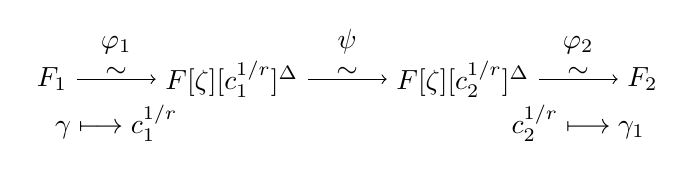
\begin{tikzpicture}
	\node (Fc1) {$F[\zeta][c_1^{1/r}]^\Delta$};
	\node[right = of Fc1] (Fc2) {$F[\zeta][c_2^{1/r}]^\Delta$};
	\node[left = of Fc1] (F1) {$F_1$};
	\node[right = of Fc2] (F2) {$F_2$};
	\draw[->] (F1) edge node[above, inner sep=0.5pt] {$\sim$} node[above = 3mm, inner 
	sep=0.5pt] {$\varphi_1$} node[below = 3mm, inner sep=0.5pt] {$\gamma \longmapsto 
		c_1^{1/r}$} (Fc1);
	\draw[->] (Fc1) edge node[above, inner sep=0.5pt] {$\sim$} node[above = 3mm, inner 
	sep=0.5pt] {$ \psi $} (Fc2);
	\draw[->] (Fc2) edge node[above, inner sep=0.5pt] {$\sim$} node[above = 3mm, inner 
	sep=0.5pt] {$ \varphi_2 $} node[below = 3mm, inner sep=0.5pt] {$c_2^{1/r} \longmapsto 
		\gamma_1$} (F2);
	\end{tikzpicture}
\end{equation*}
of isomorphisms. The following algorithm summarizes the process.
\begin{algorithm}[Lenstra]
	\begin{algorithmic}[1]
		\REQUIRE Field extensions $F_1, F_2$ of $F$ of degree $r$
		\ENSURE An isomorphism $\F_1 \xrightarrow{\sim} F_2$
		\STATE find a generator $c_i$ of $T_{F_i}$ for $i = 1, 2$
		\STATE find isomorphisms $\varphi_i: F_i \xrightarrow{\sim} F[\zeta][c_i^{1/r}]^\Delta$ for 
		$i = 1, 2$
		\STATE compute the integer $j$ such that $c_1 = c_2^j$
		\STATE build the isomorphism $\psi: F[\zeta][c_1^{1/r}]^\Delta \xrightarrow{\sim} 
		F[\zeta][c_2^{1/r}]^\Delta$
		\RETURN $\varphi_2 \circ \psi \circ \varphi_1$
	\end{algorithmic}
\end{algorithm}
A more careful look at the above approach suggests a trade-off between determinism and 
simplicity/practicality. For example, one can replace the ring extension $F[\zeta]$ with the field 
extension $F[\zeta] = F[X] / g(X)$ where $g$ is an irreducible factor of $\Phi_r$. This makes 
things simpler and more practical at the cost of factoring $\Phi_r$ which of course introduces 
indeterminism if one choses to use efficient factoring algorithms.

To find generators for the Teichm\"{u}ller subgroups, Lenstra uses some trace-like formula that 
suggests a version of Hilbert 90 Theorem over rings. Alombert's approach is more or less the same 
as above with more focus on implementation. The idea of the algorithm is to use cyclotomic field 
extensions which in turn allows a more explicit use of Hilbert 90 Theorem to find elements 
$\alpha_1 \in F_1[\zeta]$, and $\alpha_2 \in F_2[\zeta]$. Then $b = \alpha_1^r / \alpha_2^r$ is an 
$r$th power in $F[\zeta]$ from which $b^{1/r}$ can be computed using a root extraction algorithm. 
The isomorphism $F_1[\zeta] \xrightarrow{\sim} F_2[\zeta]$ is then given by $\alpha_1 \mapsto 
b^{1/r}\alpha_2$. Although again no rigorous complexity analysis is presented, one can easily see 
that the dominant cost of this algorithm is solving Hilbert 90 which is done using linear algebra. 
Therefore, the algorithm performs $O(n^{\omega + 1})$ many operations in $F$.


\subsection{Fast variant}

In this section, we present a fast variant of Allombert's algorithm using an explicit solution to 
the Hilbert 90 Theorem. Let $F = \F_q$ ,and $[k: F] = r$ where $r$ is a prime power. Let $h(Z)$ be 
an irreducible factor of the $r$-th cyclotomic polynomial over $F$. Then $h$ has degree $s$ where 
$s$ is the order of $q$ in the multiplicative group $\Z/r\Z$. We form the field extension $F(\zeta) 
\cong F[Z] / h$ and the ring extension $k[\zeta] \cong k[Z] / h \cong k \otimes F(\zeta)$ where 
$\zeta$ is the image of $Z$ in the quotients. The action of the Galois group $\gal(k / F)$ can be 
extended to $k[\zeta]$ by
\[
\begin{array}{llll}
\sigma: & k[\zeta] & \rightarrow & k[\zeta] \\
& x \otimes \zeta & \mapsto & x^q \otimes \zeta.
\end{array}
\]
Then the fixed field of $\sigma$ is $F(\zeta)$. The same can be done for the ring $K[\zeta]$. Let 
us restate the algorithm for clarity.

\begin{algorithm}[Allombert]
	\begin{algorithmic}[1]
		\REQUIRE field extensions $k, K$ of $F$ of degree $r$
		\ENSURE an isomorphism $k \xrightarrow{\sim} K$
		\STATE factor the $r$th cyclotomic polynomial and make the extensions $F(\zeta), 
		k[\zeta], K[\zeta]$
		\STATE find $\theta_1 \in k[\zeta]$ such that $\sigma(\theta_1) = \zeta\theta_1$
		\STATE find $\theta_2 \in K[\zeta]$ such that $\sigma(\theta_2) = \zeta\theta_2$
		\STATE compute an $r$th root $c$ of $\theta_1^r / \theta_2^r$ in $F(\zeta)$
		\STATE let $\alpha_1, \alpha_2$ be the constant terms of $\theta_1, c\theta_2$ respectively
		\RETURN the isomorphism $\alpha_1 \rightarrow \alpha_2$
	\end{algorithmic}
\end{algorithm}


By symmetry, we only deal with the extension $k / F$. The dominant steps of the algorithm are 
solving Hilbert 90, i.e. finding $\theta_1$, and taking an $r$-th root in $F(\zeta)$. Taking roots 
in $F(\zeta)$ can be efficiently done using the algorithm of Subsection \ref{subsection:root-Fz}. 
Replacing $v, s$ by $r, s$ respectively in Proposition \ref{proposition:root-fpz} gives the 
complexity of taking $r$-th roots in $F(\zeta)$. 

We show how to efficiently find $\theta_1$. For $a \in k[\zeta]$ define
\[ \theta_a = a + \sigma(a)\zeta^{-1} + \sigma^2(a)\zeta^{-2} + \cdots + \sigma^{r - 1}(a)\zeta^{-r 
	+ 1}. \]
We have $\sigma(\theta_a) = \zeta\theta_a$. Therefore, $\theta_a$ is a solution of Hilbert 90 over 
$k[\zeta]/F(\zeta)$. This also shows that $\theta_a^r \in F(\zeta)$. We set $\theta_1 = \theta_a$ 
for a random $a \in k[\zeta]$. If we write $\theta_1 = \sum_{i = 0}^{s - 1}f_i(x)\zeta^i$ then 
$\alpha_1 = f_0$ is what we are looking for. To compute $\theta_a$ efficiently, we take different 
approaches based on the largeness of $s$ as in Subsection \ref{subsection:root-Fz}. 

\paragraph{Small $\boldsymbol{s}$.} 
Given $a \in k[\zeta]$ define 
\[ \theta_{a, j} = a + \sigma(a)\zeta^{-1} + \cdots + \sigma^{j - 1}(a)\zeta^{-j + 1}, \quad \xi_j 
= x^{q^j}. \]
We have the following recursive relations
\[
\xi_j = 
\begin{cases}
\xi_{j / 2}^{q^{j / 2}} & j \text{ even} \\
\xi_{j - 1}^q & j \text{ odd}
\end{cases}, \quad
\theta_{a, j} = 
\begin{cases}
\theta_{a, j / 2} + \zeta^{-j / 2}\sigma^{j / 2}(\theta_{a, j / 2})& j \text{ even} \\
a + \zeta^{-1}\sigma(\theta_{a, j - 1}) & j \text{ odd}
\end{cases}
\]
Applying $\sigma^j$ to an element $b \in k[\zeta]$ is the same as composing the polynomial $b(x, 
z)$ with the polynomial $\xi_j(x)$. Algorithm \ref{algorithm:xitheta} computes $\theta_{a, 
	i}$ using above relations.

\begin{algorithm}
	[XiTheta]
	\label{algorithm:xitheta}
	\begin{algorithmic}[1]
		\REQUIRE $a \in k[\zeta]$, a positive integer $i$, $\xi_1=x^q$
		\ENSURE $\xi_i$, $\theta_{a, i}$
		\IF {$i=1$} 
		\RETURN $\xi_1$, $a$
		\ENDIF
		\STATE $j \leftarrow \lfloor i / 2 \rfloor$
		\STATE $\xi_{j},\theta_{a, j} \leftarrow {\rm XiTheta}(a, j, \xi_1)$ 
		\STATE\label{step:xij} $\xi_{2j} \leftarrow \xi_j(\xi_j)$
		\STATE\label{step:thetaj} $\theta_{a, 2j} \leftarrow \theta_{a, j} + \zeta^{-j}\theta_{a, 
			j}(\xi_j)$
		\IF {$i$ is even} 
		\RETURN $\xi_{2j}$, $\zeta_{2j}$, $\delta_{2j}$
		\ENDIF
		\STATE $\xi_i \leftarrow \xi_{2j}(\xi_1)$
		\STATE $\theta_{a, i} \leftarrow a + \zeta^{-1}\theta_{a, 2j}(\xi_1)$
		\RETURN $\xi_i$, $\theta_{a, i}$
	\end{algorithmic}
\end{algorithm}


Computing $\xi_1 = x^q$ is done using $\MM(r)\log(q)$ operations in $F$. The dominant steps of the 
algorithm are \ref{step:xij}, \ref{step:thetaj}. Step \ref{step:xij} takes one modular composition 
at the cost of $\CC(r)$ operations in $F$. Using the representation $a = \sum_{i = 0}^{s - 
	1}a_i(x)\zeta^i$ for an element $a \in k[\zeta]$, Step \ref{step:thetaj} takes $O(s)$ modular 
compositions over $F$ at the total cost of $O(s\CC(r))$ operations in $F$. Computing $\theta_a = 
\theta_{a, r}$ needs a recursion of depth $O(\log(r))$, and hence a total cost of $O(s\CC(r)\log(r) 
+ \MM(r)\log(q))$ operations in $F$.

\paragraph{Large $\boldsymbol{s}$.}
Consider the restrictions $\sigma^i \vert_{k^*}: k^* \rightarrow k[\zeta]^*$. Adapting the same 
idea of the proof \cite[Ch VI, Theorem 4.1]{lang}, one checks that these mappings are linearly 
independent. Therefore, there is $a(x) \in k^*$ such that 
\[ \theta_a = a(x) + a(x)^q\zeta^{-1} + a(x)^{q^2}\zeta^{-2} + \cdots + a(x)^{q^{r - 1}}\zeta^{-r 
	+ 1}\]
is not zero. Given $x^q$, the sequence $a(x), a(x)^q, \dots, a(x)^{q^{(r - 1)}}$ in $k$ can be 
computed by Algorithm 3.1 in \cite{von1992computing} using $O(\MM(r^2)\log(r))$ operations in $F$. 
Putting the above cases together we have
\begin{proposition}
	\label{proposition:XiDelta-updated}
	Finding a nonzero $\theta_a$ for random $a \in k[\zeta]$ takes
	\begin{itemize}
		\item $O(s\CC(r)\log(r) + \MM(r)\log(q))$ operations in $F$ for small $s$, or
		\item $O(\MM(r^2)\log(r) + \MM(r)\log(q))$ operations in $F$ for large $s$.
	\end{itemize}
\end{proposition}

Combining this with the cost of taking roots in $F(\zeta)$ we get the following for the cost of 
computing an embedding $k \hookrightarrow K$.

\begin{proposition}
	\label{proposition:XiDelta-updated}
	Computing an embedding $k \hookrightarrow K$ takes
	\begin{itemize}
		\item $O(s\CC(r)\log(r) + \MM(r)\log(q))$ operations in $F$ for small $s$, or
		\item $O(\MM(r^2)\log^2(r) + \MM(r)\log(r)\log(q))$ operations in $F$ for large $s$.
	\end{itemize}
\end{proposition}




\subsubsection{The Artin-Schreier case}
\label{sec:artin-schreier-case}

\todo{We have to write at least a few paragraphs on how to handle this case.}

%%%%%%%%%%%%%%%%%%%%%%%%%%%%%%%%%%
\section{Rains' algorithm}

We now move on to a family of algorithms based on the theory of
algebraic groups. The simplest of these algorithms is Pinch's
cyclotomic algorithm~\cite{Pinch}. The idea is very simple: given $r$,
select an integer $\ell$ such that $[\F_q[\mu_\ell]:\F_q]=r$, where
$\mu_\ell$ is the group of $\ell$-th roots of unity.  Then, any
embedding $k\to K$ takes $\mu_\ell\subset k^\ast$ to $\mu_\ell\subset
K^\ast$, and the minimal polynomial of any primitive $\ell$-th root of
unity has degree exactly $r$.

Pinch's algorithm is very effective when $r=\euler(\ell)$. Indeed in
this case the $\ell$-th cyclotomic polynomial $\Phi_\ell$ is
irreducible over $\F_q$, and its roots form a unique orbit under the
action of the absolute Galois group of $\F_q$. Thus we can take any
primitive $\ell$-th roots of unity $\alpha\in k$ and $\beta\in K$ to
describe the embedding.

In the general case, however, the roots of $\Phi_\ell$ are partitioned
in $\euler(\ell)/r$ orbits, thus for two randomly chosen $\ell$-th
roots of unity $\zeta_1\in k$ and $\zeta_2\in K$, we can only say that
there exists an exponent $e$ such that
\begin{equation*}
  \alpha = \zeta_1 \mapsto \zeta_2^e = \beta
\end{equation*}
defines a valid embedding. Pinch's algorithm tests all possible
exponents $e$, until a suitable one is found. To test for the validity
of a given $e$, it applies the embedding $\phi:\zeta_1\mapsto\zeta_2$
to the class of $X$ in $k$, and verfies that its image is a root of
$f$ in $K$ (see Part~\ref{part:eval} for details on embedding
evaluation).

The trial-and-error nature of Pinch's algorithm makes it impractical,
except for rare favorable cases where a \emph{small} $\ell$ such that
$r=\euler(\ell)$ can be found. One possible workaround, suggested by
Pinch himself, is to replace the group of roots of unity with a group
of torsion points of a well chosen elliptic curve. We analyze this
idea in greater detail in Section~\ref{sec:rains-elliptic}.

This section is devoted to a different way of improving Pinch's
algorithm, imagined by Rains~\cite{rains2008}, and implemented in the
Magma computer algebra system~\cite{MAGMA}. Rains' original preprint
went unpublished\footnote{The only publicly available source for
  Rains' algorithm is Magma's source code (file
  \texttt{package/Ring/FldFin/embed.m}, since v2.14).}, thus we
describe his algorithm in detail for completeness. Rains' technical
contribution is twofold: first he replaces roots of unity with
Gaussian periods to avoid trial-and-error, second he moves to slightly
larger extension fields to ensure the existence of a small $\ell$ as
above.

\subsection{Uniquely defined orbits from Gaussian periods}

For the rest of the section, we are going to assume that $q$ is
prime. The case where $q$ is a higher power of a prime is discussed in
Note~\ref{note:rains-non-prime}.

Suppose that we have an $\ell$, coprime with $q$, such that
$[\F_q[\mu_\ell]:\F_q]=r$, then the cyclotomic polynomial $\Phi_\ell$
factors over $\F_q$ into $\euler(\ell)/r$ distinct factors of degree
$r$. Pinch's method, by choosing random roots of $\Phi_\ell$ in $k$
and $K$, randomly selects one of these factors as minimal polynomial.

By combining the roots of $\Phi_\ell$ into Gaussian periods, Rains'
method uniquely selects a minimal polynomial of degree $r$. The
construction is best understood by looking at the Galois groups of
cyclotomic fields. It is well known that the Galois group of
$\Q[\mu_\ell]/\Q$ is canonically isomorphic to $(\Z/\ell\Z)^\ast$ via
the mapping
\begin{equation*}
  \begin{aligned}
    (\Z/\ell\Z)^\ast &\to \gal(\Q[\mu_\ell]/\Q),\\
    e &\mapsto (\sigma_e : \zeta_\ell\mapsto\zeta_\ell^e),
  \end{aligned}
\end{equation*}
where $\sigma_e$ is the map sending any $\ell$-th root of unity to its
$e$-th power, extended by linearity to all of $\Q[\mu_\ell]$. Gaussian
periods are defined as traces of generators of $\mu_\ell$ down to a
subfield of $\Q[\mu_\ell]$.

\begin{definition}
  Let $S$ be a subgroup of $(\Z/\ell\Z)^\ast$, and let $L$ be the
  subfield of $\Q[\mu_\ell]$ fixed by $S$. For any generator
  $\zeta_\ell$ of $\mu_\ell$, define the Gaussian period
  $\eta(\zeta_\ell)$ as
  \begin{equation}
    \eta(\zeta_\ell) = \trace_{\Q[\mu_\ell]/L} \zeta_\ell = \sum_{\sigma\in S}{\zeta_\ell^{\sigma}}.
  \end{equation}
\end{definition}

By hypothesis, the prime $q$ factors as a product of $\euler(\ell)/r$
distinct primes ideals in $\Z[\mu_\ell]$. Let $\mathfrak{q}$ be one
such prime ideal, then $\F_q[\mu_\ell]$ is isomorphic to the residue
field $\Z[\mu_\ell]/\mathfrak{q}$, and we can identify (canonically)
the Galois group $\gal(\F_q[\mu_\ell]/\F_q)$ with the subgroup
$\langle q\rangle\subset(\Z/\ell\Z)^\ast$.

Now, suppose there is a group $S$ such that
$(\Z/\ell\Z)^\ast=\langle q\rangle\times S$, let $L$ be the field fixed
by $S$, and let $\mathcal{O}_L$ be its ring of integers. Then, the
Galois group of $L/\Q$ is also canonically identified with $\langle
q\rangle\subset(\Z/\ell\Z)^\ast$, the prime $q$ is inert in $L$, and
$\mathcal{O}_L/q\mathcal{O}_L$ is isomorphic to
$\F_q[\mu_\ell]$. While the identification of $\F_q[\mu_\ell]$ with
$\Z[\mu_\ell]/\mathfrak{q}$ depended on the choice of the prime
$\mathfrak{q}$, taking the trace down to $L$ and then reducing modulo
$q$ is independent of such choice, we obtain thus a canonical
identification between $\mathcal{O}_L/q\mathcal{O}_L$ and
$\F_q[\mu_\ell]$. The situation is summarized in the following
diagram:
\begin{equation*}
  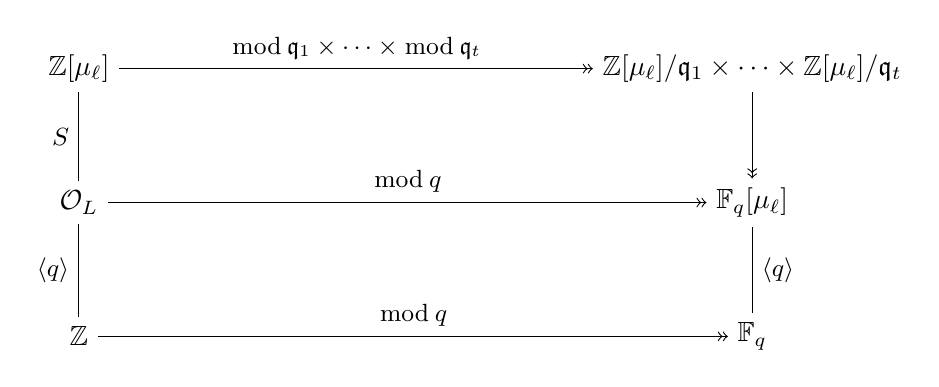
\begin{tikzpicture}[node distance=1.7cm]
    \node (Q) {$\Z$};
    \node[above of=Q] (L) {$\mathcal{O}_L$};
    \node[above of=L] (Qm) {$\Z[\mu_\ell]$};
    \node[right=8cm of Q] (Fp) {$\F_q$};
    \node[above of=Fp] (Fpm) {$\F_q[\mu_\ell]$};
    \node[above of=Fpm] (Prod) {$\Z[\mu_\ell]/\mathfrak{q}_1\times\cdots\times\Z[\mu_\ell]/\mathfrak{q}_t$};
    \draw 
    (Q) edge node[left] {\small $\langle q\rangle$} (L)
    (L) edge node[left] {\small $S$} (Qm)
    (Fp) edge node[right] {\small $\langle q\rangle$} (Fpm); 
    \draw[->>] 
    (Q) edge node[above] {\small $\bmod\, q$} (Fp)
    (L) edge node[above] {\small $\bmod\, q$} (Fpm)
    (Qm) edge node[above] {\small $\bmod\, \mathfrak{q}_1\times\cdots\times\bmod\,\mathfrak{q}_t$} (Prod)
    (Prod) edge node[right] {} (Fpm);
  \end{tikzpicture}
\end{equation*}

We can now extend the definition of Gaussian period to finite fields.

\begin{definition}
  Suppose that there is a subgroup $S\subset(\Z/\ell\Z)^\ast$ such
  that $(\Z/\ell\Z)^\ast=\langle q\rangle\times S$. For any generator
  $\zeta_\ell$ of $\mu_\ell$ in $\F_q[\mu_\ell]$, define the Gaussian
  period $\eta_q(\zeta_\ell)$ as
  \begin{equation}
    \eta_q(\zeta_\ell) = \sum_{\sigma\in S}{\zeta_\ell^{\sigma}}.
  \end{equation}
\end{definition}

\begin{lemma}
  \label{th:gaussian}
  Let $\ell$ be a squarefree integer such that $(\Z/\ell\Z)^\ast =
  \langle q\rangle \times S$ for some $S$.  The periods
  $\eta_q(\zeta_\ell^\sigma)$ for $\sigma$ running through $\langle
  q\rangle$ form a normal basis of $\F_q[\mu_\ell]$ over $\F_q$,
  independent of the choice of $\zeta_\ell$.
\end{lemma}
\begin{proof}
  See~\cite[Main Theorem]{feisel1999normal}.
\end{proof}

In what follows we are going to write $\eta(\zeta_\ell)$ when $q$ is
clear from the context.

\begin{example} 
  Consider the extension $\F_8/\F_2$ of degree $3$, which is generated
  by the $7$-th roots of unity. We have a decomposition
  $(\Z/7\Z)^\ast=\langle 2\rangle\times\langle-1\rangle$, and the
  cyclotomic polynomial factors as
  \begin{equation}
    \Phi_7(x) = (x^3 + x + 1) (x^3 + x^2 + 1).
  \end{equation}
  For any root $\zeta_7$, we define the period
  \begin{equation}
    \eta_2(\zeta_7) = \zeta_7+\zeta_7^{-1}.
  \end{equation}
  The three periods $\eta_2(\zeta_7)$, $\eta_2(\zeta_7)^2$ and
  $\eta_2(\zeta_7)^4$ are all roots of the polynomial $x^3+x^2+1$ and
  form a normal basis of $\F_8/\F_2$.
\end{example}

\subsection{Rains' cyclotomic algorithm}

The bottom-line of Rains' algorithm follows immediately from the
previous section: given $k$, $K$ and $r$,
\begin{enumerate}
\item find a \emph{small} $\ell$ satisfying the conditions of
  Lemma~\ref{th:gaussian} with $[\F_q[\mu_\ell]:\F_q]=r$;
\item take random $\ell$-th roots of unity $\zeta_\ell\in k$ and
  $\zeta_\ell'\in K$;
\item return the Gaussian periods $\alpha_r=\eta(\zeta_\ell)$ and
  $\beta_r=\eta(\zeta_\ell')$.
\end{enumerate}

The problem with this algorithm is the vaguely defined
\emph{smallness} requirement on $\ell$. Indeed the conditions of
Lemma~\ref{th:gaussian} imply that $\ell$ divides $\Phi_r(q)$, thus in
the worst case $\ell$ can be as large as $O(q^{\euler(r)})$, which
yields an algorithm of exponential complexity in the field size.

To circumvent this problem, Rains allows the algorithm to work in
small auxiliary extensions of $k$ and $K$, and then descend the
results to $k$ and $K$ via a field trace. In other words, Rains'
algorithm looks for $\ell$ such that $[\F_q[\mu_\ell]:\F_q]=rs$ for
some small $s$. We summarize this method in
Algorithm~\ref{algorithm:rains-cyclo}; we only give the procedure for
the smaller field $k$, the procedure for the larger field $K$ being
identical.

\begin{algorithm}[Rains' cyclotomic algorithm]
  \label{algorithm:rains-cyclo}
  \begin{algorithmic}[1]
    \REQUIRE A field extension $k/\F_q$ of degree $m$, a prime power
    $r|m$, a prime $\ell$ such that
    \begin{itemize}
    \item $(\Z/\ell\Z)^\ast = \langle q\rangle \times S$ for some $S$,
    \item $\#\langle q\rangle = rs$ for some integer $s$.
    \end{itemize}
    \ENSURE A normal generator of $\F_{q^r}\subset k$ over $\F_q$,
    with a uniquely defined Galois orbit.
    
    \STATE Construct the smallest field extension $k'/k$
    containing $\F_{q^{rs}}$; 
    \REPEAT
    \STATE Compute $\zeta = \theta^{(\#k'-1)/\ell}$ for a random $\theta\in k'$
    \UNTIL $\zeta$ is a primitive $\ell$-th root of unity;
    \STATE\label{algorithm:rains-cyclo:period} Compute $\eta(\zeta) = \sum_{\sigma\in S}\zeta^\sigma$;
    \RETURN\label{algorithm:rains-cyclo:trace} $\alpha_r = \trace_{\F_{q^{rs}}/\F_{q^r}}\eta(\zeta) = \sum_{i=0}^{s-1}\eta(\zeta)^{q^{ri}}$.
  \end{algorithmic}
\end{algorithm}

\begin{proposition}
  Algorithm~\ref{algorithm:rains-cyclo} is correct. On input
  $m,q,r,\ell,s$ it computes its output using $O(\MM(ms)(ms\log q +
  (\ell\log\ell)/r))$ operations in $\F_q$, or $\tildO(m^2s^2\log q)$
  assuming $\ell\in o(mrs)$.
\end{proposition}
\begin{proof}
  By construction $k'$ contains a subfield isomorphic to $\F_{q^{rs}}$
  and to $\F_q[\mu_\ell]$. By Lemma~\ref{th:gaussian} $\eta(\zeta)$ is
  a normal generator of $\F_{q^{rs}}$, and
  by~\cite[Prop.~5.2.3.1]{mullen2013handbook} $\alpha_r$ is a normal generator of
  $\F_{q^r}\subset k$.

  In the worst case $[k':k]=s$. Using the techniques
  in~\cite{couveignes+lercier11,DeDoSc13,DeFeo:2014:FAA:2608628.2608672},
  $k'$ can be constructed, and elements can be moved between $k$ and
  $k'$ using $O(\MM(ms))$ operations in $\F_q$ \todo{This is very
    optimistic, esp. if $s$ is not coprime to $m$}.

  The root of unity $\zeta$ is obtained after $O(1)$ tries on average,
  at a cost of $O(\MM(ms)ms\log q)$ operations each.
  Steps~\ref{algorithm:rains-cyclo:period}
  and~\ref{algorithm:rains-cyclo:trace} can be performed at once by
  observing that
  \[\alpha_r = \sum_{i=0}^{s-1}\eta(\zeta^{q^{ri}})= \sum_{i=0}^{s-1}\sum_{\sigma\in S}\zeta^{q^{ri}\sigma}.\]
  By reducing $q^{ri}\sigma$ modulo $\ell$, we can compute this sum at
  the cost of $\euler(\ell)/r$ exponentiations of degree at most
  $\ell$ in $k'$, for a total cost of $O((\MM(ms)\ell\log\ell)/r)$.
\end{proof}

We now present a variant of Rains' algorithm which avoids the
construction of the field extension $k'$. 

\begin{algorithm}[Rains' cyclotomic algorithm variant]
  \label{algorithm:rains-cyclo-2}
  \begin{algorithmic}[1]
    \REQUIRE A field extension $k/\F_q$ of degree $m$, a prime power
    $r|m$, a prime $\ell$ such that
    \begin{itemize}
    \item $(\Z/\ell\Z)^\ast = \langle q\rangle \times S$ for some $S$,
    \item $\#\langle q\rangle = rs$ for some integer $s$.
    \end{itemize}
    \ENSURE A normal generator of $\F_{q^r}\subset k$ over $\F_q$,
    with a uniquely defined Galois orbit.
    
    \STATE Compute a factor $h$ of the $\ell$-th cyclotomic polynomial $\Phi_\ell$ in $k[Z]$ using Algorithm~\ref{alg:cyclo}; 
    \STATE Compute $\bar{h} \leftarrow \rev{h'}/\rev{h} \bmod Z^\ell$;
    \STATE Let $s'=\gcd(s,m/r)$ and $S' = \langle q^{rs/s'}\rangle \times S$;
    \RETURN\label{algorithm:rains-cyclo:period} $\eta \leftarrow -\sum_{\sigma\in S'}[\bar{h}]_\sigma$.
  \end{algorithmic}
\end{algorithm}


\begin{proposition}
  Algorithm~\ref{algorithm:rains-cyclo} is correct. On input
  $m,q,r,\ell,s$ it computes its output using $O(\ell
  m(\log(s)+\log(m))\log(\ell) + \MM(\ell m)\log(\ell m) + \MM(\ell
  m)\log(q))$ operations in $\F_q$.
\end{proposition}
\begin{proof}
  Factoring $\Phi_\ell$ costs $O(\ell m(\log(s)+\log(m))\log(\ell) +
  \MM(\ell m)\log(\ell m) + \MM(\ell m)\log(q))$ according to
  Prop.~\ref{th:cyclo}.

  $\bar{h}$ is computed by a Euclidean division in $O(\MM(\ell m))$
  operations. The final sum is computed in $O(\ell m)$ operations.
\end{proof}


This concludes the presentation of Rains' algorithm. However, we are
still left with a problem: how to find $\ell$ satisfying the
conditions of the algorithm, and what bounds can be given on it. These
questions will be analyzed in Section~\ref{sec:selection}.

\begin{remark}
  Various practical optimizations are possible for Rains'
  algorithm. We list here some of them.
  \begin{itemize}
  \item If $s$ cannot be chosen so that $k'=k$, then it is interesting
    to take $s$ coprime with $m$. In this case, the extension $k$' can
    be built using a polynomial with coefficients in $\F_q$ rather
    than $k$, and a lookup table of irreducible polynomials can be
    established for small $s$.
  \item Different prime powers $r_1,r_2,\dots$ can be treated
    simultaneously in some cases. We come back to this in
    Section~\ref{sec:selection}.
  \item In some cases, the trace in the final step can be computed
    more efficiently by exploiting the fact that it is a linear form,
    as per~\cite{todo}.
  \end{itemize}
\end{remark}

\begin{note}
  \label{note:rains-non-prime}
  Rains' algorithm is easily extended to a non-prime field $\F_q$, as
  long as $q=p^d$ with $\gcd(d,r)=1$. In this case, indeed, any
  generator of $\F_{p^r}$ over $\F_p$ is also a generator of
  $\F_{q^r}$ over $\F_q$. The algorithm is unchanged, except for the
  additional requirement that $\gcd(\euler(\ell),d)=1$, which ensures
  that the Gaussian periods indeed generate $\F_{p^r}$.

  However, when $\gcd(d,r)\ne 1$, it is impossible to have
  $(\Z/\ell\Z)^\ast=\langle q\rangle\times S$, so Rains' algorithm
  simply cannot be applied to this case. In the next section we are
  going to present a variant that does not suffer from this problem.
\end{note}


%%%%%%%%%%%%%%%%%%%%%%%%%%%%%%%%%%

\section{Elliptic Rains' algorithm}
\label{sec:rains-elliptic}

The Pinch/Rains' algorithm presented in the previous section relies on the use
of the multiplicative group of finite fields.
It is natural to try to extend it to other types of algebraic groups in
order to cover a wider range of parameters.
And indeed Pinch~\cite{Pinch} showed how to use torsion points of elliptic
curves in place roots of unity.
Rains also considered this possiblity, but did not investigate it thoroughly
as no theoretical gain was to be expected.
However, the situation in practice is quite different.
In particular, the need for auxiliary extensions in the cyclotomic method
is very costly, whereas the elliptic variant naturally works in the input 
fields, and is therefore very competitive.

In the next sections, we first introduce \emph{elliptic periods}, a
straightforward generalization of Gaussian periods for torsion points
of elliptic curves, the non-trivial part being to show that
elliptic periods yield (power) bases of finite fields,
then analyze the cost of their computation.

\subsection{Uniquely defined orbits from elliptic periods}

Throughout this section $q$ is an odd prime power. 

An elliptic curve $E/L$ defined over a field $L$ of characteristic
$>2$ is an equation of the form
\begin{equation*}
  E\;:\; y^2 = x^3 + a_2x^2 + a_4x + a_6
  \qquad\text{with $a_2,a_4,a_6\in L$.}
\end{equation*}
For any field extension $M/L$ the group of $M$-rational points of $E$
is the set
\begin{equation*}
  E(M) = \{(x,y)\in M^2 \mid E(x,y) = 0\} \cup \{\mathcal{O}\}
\end{equation*}
endowed with the usual group law.

For an integer $\ell$, we denote by $E[\ell]$ the $\ell$-torsion
subgroup of $E(\bar{L})$, where $\bar{L}$ denotes the algebraic
closure of $L$. In this section we are going to consider integers
$\ell$ coprime with the characteristic of $L$, then $E[\ell]$ is a
group of rank $2$.

For an elliptic curve $E/\F_q$ defined over a finite field, we denote
by $\pi$ its \emph{Frobenius endomorphism}. It is well known that
$\pi$ satisfies a quadratic equation $\pi^2-t\pi+q=0$, where $t$ is
called the \emph{trace of $E$}, and that this equation determines the
cardinality of $E$ as $\#E(\F_q)=q+1-t$.

Like in the cyclotomic case, the Frobenius endomorphism partitions
$E[\ell]$ into orbits. Our goal is to take traces of points in
$E[\ell]$ so that a uniquely defined orbit arises. This task is made
more complex by the fact that $E[\ell]$ has rank 2, hence we are going
to restrict to a family of primes $\ell$ named \emph{Elkies primes}.

\begin{definition}[Elkies prime]
  Let $E/\F_q$ be an elliptic curve, let $\ell$ be a prime number not
  dividing $q$.  We say that $\ell$ is an Elkies prime for $E$ if the
  characteristic polynomial of the Frobenius endomorphism $\pi$ splits
  into two distinct factors over $\Z/\ell\Z$:
\begin{equation}
\pi^2-t\pi+q=(\pi-\lambda)(\pi-\mu)\bmod\ell
\qquad\text{with $\lambda\ne\mu$}.
\end{equation}
\end{definition}

Note that if $\ell$ is an Elkies prime for $E$,
then $E[\ell]$ splits into two eigenspaces for $\pi$
which are defined on extensions of $\F_q$ of degrees
$\order_\ell(\lambda)$ and $\order_\ell(\mu)$.

Another subtlety arises in comparison with multiplicative groups:
elliptic curves always come with non trivial automorphisms. We recall
that the size of the \emph{group of rational automorphisms} of a curve
$E/\F_q$ is one of the following:
\begin{itemize}
\item $\#\Aut_{\F_q}(E) = 12$ if $j(E)=0$ and $q=0\mod 9$ \todo{is this correct? useful?},
\item $\#\Aut_{\F_q}(E) = 6$ if $j(E)=0$ and $q=1\mod 3$,
\item $\#\Aut_{\F_q}(E) = 4$ if $j(E)=1728$ and $q=1\mod 4$,
\item $\#\Aut_{\F_q}(E) = 2$ otherwise.
\end{itemize}

\begin{definition}
\label{definition:ellperiod}
Let $E/\F_q$ be an elliptic curve, with $j(E)\ne0$ if $3|q$.
Let $\ell > 3$ be an Elkies prime for $E$,
$\lambda$ an eigenvalue of $\pi$ such that $\order_\ell(\lambda)$ is odd,
and $P \in E[\ell]$ a point in the eigenspace corresponding
to $\lambda$.

Let $A=\Aut_{\F_q}(E)$, and suppose that $\# A$ divides $\ell - 1$,
and that there is a subgroup $S$ of $(\Z/\ell\Z)^{\ast}$ such that
\begin{equation}
(\Z/\ell\Z)^{\ast} / A = \langle{\lambda}\rangle \times S.
\end{equation}

Then we define an elliptic period as
\begin{equation}
\eta_\lambda(P) = \sum_{\sigma\in S} {x \left([\sigma] P \right)^{\# A/2}},
\end{equation}
where $x(P)$ denotes the abscissa of $P$.
\end{definition}

\begin{theorem}
\label{theorem:ellperiods}
Let $\ell$ be a prime not dividing $q$, and let $t, \lambda, \mu$ be
integers such that
\begin{enumerate}
    \item $\lvert t \rvert < \sqrt{2q}$,
    \item $X^2 - tX + q = (X - \lambda)(X - \mu)\bmod \ell$,
    \item $(\Z/\ell\Z)^{\ast}/\Aut_{\F_q}(E) = \langle{\lambda}\rangle \times S$
for $S$ a subgroup of $(\Z/\ell\Z)^{\ast}$.
\end{enumerate}

Let $E/\F_q$ be an elliptic curve of trace $t$
and $P \in E[\ell]$ a point in the eigenspace
corresponding to $\lambda$.

Then the elliptic period $\eta_\lambda(P)$ generates $\F_q[x(P)]$ over
$\F_q$.  Furthermore, the Galois orbit of $\eta_\lambda(P)$ is
independent of the choice of $P$.
\end{theorem}

\begin{proof}
We are not sure this is true!
For sure, $\eta_\lambda(P)$ is not a normal element (in general).
I'll gather some known facts here.
Here is the rainbow diagram.
\begin{center}
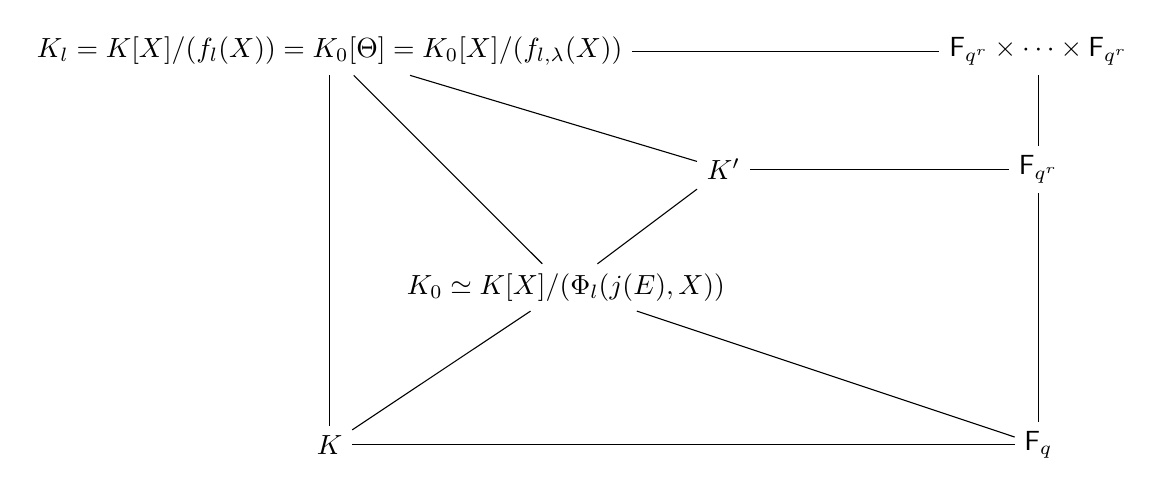
\begin{tikzpicture}
\node (Kl) {$K_l = K[X] / (f_l(X)) = K_0[\Theta] = K_0[X] / (f_{l, \lambda}(X))$};
\node [below of=Kl, node distance=3cm, align=center] (KlK) {};
\node [below of=KlK, node distance=2cm, align=center] (K) {$K$};
\node [right of=KlK, node distance=3cm] (K0) {$K_0 \simeq K[X]/(\Phi_l(j(E), X))$};
\node [right of=K0, yshift=+1.5cm, node distance=2cm] (Kp) {$K'$};
\node [right of=K0, yshift=-2cm, node distance=+6cm] (Fq) {$\mathsf{F}_q$};
\node [right of=Kp, node distance=+4cm] (Fqr) {$\mathsf{F}_{q^r}$};
\node [above of=Fqr, node distance=+1.5cm, align=center] (Fqrs) {$\mathsf{F}_{q^r} \times \cdots \times \mathsf{F}_{q^r}$};
\draw (Kl) -- (K);
\draw (K) -- (K0);
\draw (K0) -- (Kl);
\draw (K0) -- (Kp);
\draw (Kp) -- (Kl);
\draw (Kp) -- (Fqr);
\draw (Fq) -- (Fqr);
\draw (Fqr) -- (Fqrs);
\draw (Kl) -- (Fqrs);
\draw (K0) -- (Fq);
\draw (K) -- (Fq);
\end{tikzpicture}
\end{center}
\end{proof}

\subsection{Elliptic variant of Rains' algorithm}

Rain's cyclotomic algorithm needs auxiliary extensions to accommodate
for sufficiently small subgroups $\mu_\ell$ of the unit group. By
replacing unit groups with torsion groups of elliptic curves, we gain
more freedom on the choice of the size of the group, thus we are able
to work with smaller fields.  

The algorithm is very similar to
Algorithm~\ref{algorithm:rains-cyclo}, and follows immediately from
the previous section. Given $k$, $K$ and $r$,
\begin{enumerate}
\item find a prime $\ell$, an elliptic curve $E$, and an eigenvalue
  $\lambda$ of the Frobenius endomorphism, satisfying the conditions
  of Theorem~\ref{theorem:ellperiods}, and such that
  $\order_\ell(\lambda)=r$;
\item take random points $P\in E(k)[\ell]$ and $P'\in E(k')[\ell]$ in
  the eigenspace of $\lambda$;
\item return the elliptic periods $\alpha_r := \eta_{\lambda}(P)$ and
  $\beta_r:= \eta_\lambda(P')$.
\end{enumerate}

Here we are faced with a difficulty: given $E$ and $\lambda$ it is
easy to pick a random point in $E[\ell]$, but it is potentially much
more expensive to compute a point in the eigenspace of $\lambda$. We
will circumvent the problem by forcing $E(\F_{q^r})[\ell]$ to be of
rank $1$, and to coincide exactly with the eigenspace of $\lambda$.
If we write $\mu = q/\lambda$ for the other eigenvalue of $\pi$, this
is easily ensured by further asking that $\order_\ell(\mu) \nmid r$.

We defer the discussion on the search for the elliptic curve $E$ to
Section~\ref{sec:selection}. Here we suppose we are already given
suitable parameters $\ell$, $E$ and $\lambda$, and analyze the last
two steps of the algorithm, summarized below.  We only give the
procedure for the smaller field $k$, the procedure for the larger
field $K$ being identical.

\begin{algorithm}[Elliptic Rain's algorithm]
\label{algorithm:compell}
  \begin{algorithmic}[1]
    \REQUIRE An odd integer $r$, a field extension $\F_{q^r}/\F_q$,
    an elliptic curve $E/\F_q$, its trace $t$, a prime $\ell$ not dividing $q$,
    an integer $\lambda$ such that:
    \begin{itemize}
    \item $X^2 - tX - q = (X-\lambda)(X-q/\lambda) \mod\ell$,
    \item $\order_\ell(\lambda)=r$, $\order_\ell(q/\lambda)\nmid r$,
    \item $(\Z/\ell\Z)^{\ast}/\Aut_{\F_q}(E) = \langle{\lambda}\rangle \times S$ for some $S$.
    \end{itemize}
    \ENSURE A generator of $\F_{q^r}\subset k$ over $\F_q$, with a uniquely defined Galois orbit.
    \REPEAT
    \STATE Compute $P\leftarrow[\# E(\F_{q^r})/\ell]Q$ for a random $Q\in E(\F_{q^r})$;
    \UNTIL{$P\neq\mathcal{O}$;}
    \RETURN $\alpha_r\leftarrow\eta_\lambda(P)$.
  \end{algorithmic}
\end{algorithm}

\begin{proposition}
  Algorithm (\ref{algorithm:compell}) is correct. On input
  $r,q,E,t,\ell,\lambda$ it computes its output using
  $O(\MM(r)(r\log{q} + (\ell/r)\log{\ell})$ operations in $\F_q$, or
  $\tildO(r^2\log q)$ assuming $\ell\in o(r^2)$.
\end{proposition}
\begin{proof}
  By construction the point $P$ has $r$ distinct conjugates in
  $\F_{q^r}$, and, since $r$ is odd, all have distinct abscissas,
  hence $x(P)$ generates $\F_{q^r}$.  The correctness of the algorithm
  then follows immediately from Theorem~\ref{theorem:ellperiods} and
  the discussion above.

  From the knowledge of the trace $t$, we immediately determine the
  zeta function of $E$, and hence the cardinality $\# E(\F_{q^r})$, at
  no algebraic cost.

  To select the random point $Q\in E(\F_{q^r})$ we take a random
  element $x\in\F_{q^r}$, then we verify that it is the abscissa of a
  point using a squareness test, at a costs of $O(r\MM(r)\log q)$
  operations. Then, using Montgomery's formulas for scalar
  multiplication~\cite{montgomery}, we can compute the points $P$ and
  $[\ell]P$ without the knowledge of the ordinate of $Q$, at a cost of
  $O(r\MM(r)\log q)$ operations. A valid point is obtained after
  $O(1)$ tries on average.

  The elliptic period in the final step requires $O(\ell/r)$ scalar
  multiplications by an integer less than $\ell$, for a total cost of
  $O((\MM(r)\ell\log\ell)/r)$.
\end{proof}


\section{Algorithm selection}
\label{sec:selection}

The algorithms presented in the previous sections have very similar
complexities, and no one stands out as absolute winner. The complexity
of all algorithms, besides the naive one, depends in a non-trivial way
on the parameters $q$ and $r$, and, for Rains' algorithms, on the
search for a parameter $\ell$ and an associated elliptic curve.

This section studies the complexity of the embedding description
problem from a global perspective. We give procedures to find
parameters for Rains' algorithms, criteria to choose the best among
the embedding algorithms, and asymptotic bounds on the embedding
description problem.


\subsection{Finding parameters for Rains' algorithms}

Given parameters $q$ and $r$, Rains' cyclotomic algorithm asks for a
\emph{small} parameter $\ell$ such that:
\begin{enumerate}
\item $(\Z/\ell\Z)^\ast = \langle q\rangle \times S$ for some $S$,
\item $\langle q \rangle = rs$ for some integer $s$.
\end{enumerate}

Since $r$ is a prime power, the second condition lets us take a prime
power for $\ell$ too. Indeed if
$\Z/\ell\Z\simeq\Z/\ell_1\Z\times\Z/\ell_2\Z$, then either
$q\bmod\ell_1$ or $q\bmod\ell_2$ has order a multiple of $r$.
Furthermore, if $\gcd(\ell,r)=1$, then we can take $\ell$ prime, since
higher powers would not help satisfy the conditions. On the other
hand, if $\gcd(\ell,r)\ne1$, then Kummer-type algorithms have better
complexity \todo{double-check this}, hence we shall take $\ell$ prime.

Given the above constraints, we can rewrite the conditions as:
\begin{enumerate}
\item $\ell = rsu + 1$ for some $s,u$ such that $\gcd(rs,u)=1$,
\item $\order_\ell(q) = rs$.
\end{enumerate}

\begin{remark}
  Rains remarked that, when $q=2$ and $r$ is a power of $2$ greater
  than $4$, no $\ell$ can satisfy these constraints because $2$ is a
  quadratic residue modulo any prime of the form $8u+1$. This case,
  however, is covered by the Artin-Schreier technique in
  Section~\ref{sec:artin-schreier-case}, we thus ignore it.
\end{remark}

In the elliptic algorithm we look for an integer $\ell$ and a curve
$E/\F_q$ that satisfy the preconditions of
Algorithm~\ref{algorithm:compell}, i.e., such that 
\begin{enumerate}
\item the Frobenius endomorphism $\pi$ satisfies a characteristic
  equation $(\pi-\lambda)(\pi-\mu) = 0 \mod \ell$,
\item $(\Z/\ell\Z)^\ast = \langle\lambda\rangle\times T$ for some $T$,
\item $\#\langle\lambda\rangle=r$, and
\item $\mu^r\ne1\mod\ell$.
\end{enumerate}

As before, we only need to look at prime $\ell$. For simplicity, we
also exclude the case where $r$ is a power of $2$, which is easily
dealt with Kummer-type algorithms. Because $\mu=q/\lambda$, the last
condition is equivalent to $q^r\ne1\bmod\ell$. Hence, we can restate
the conditions on $\ell$ as
\begin{enumerate}
\item $\ell = ru+1$ for some $u$ such that $\gcd(r,u)=1$,
\item $q^r\ne1\mod\ell$.
\end{enumerate}
Once $\ell$ is found, we compile a list of all integers of order $r$
in $(\Z/\ell\Z)^\ast$, and look for a curve of trace
$t=\lambda+q/\lambda\bmod\ell$ for any $\lambda$ in the list. Note,
however, that for there to be such a curve, $t$ must have a
representative in the interval $[-2\sqrt{q},2\sqrt{q}]$. In order to
have a good chance of finding such curves, we are going to require
$\ell\ll\sqrt{q}$.

We propose a procedure to simultaneously find parameters for the
cyclotomic and the elliptic case in
Algorithm~\ref{algorithm:selectell}. The procedure is given bounds on
the size of the parameters sought, and outputs all suitable parameters
within those bounds.

\begin{algorithm}
    [Parameter selection for Rains' algorithms]
    \label{algorithm:selectell}
    \begin{algorithmic}[1]
      \REQUIRE Integers $q$ and $r$, bounds $\bar{u}$, $\bar{s}$, and $\bar{e}\ll\sqrt{q}$;
      \ENSURE $\mathcal{C}$ and $\mathcal{E}$, lists of parameters for the cyclotomic and elliptic algorithm resp.
      \STATE $\mathcal{C}\leftarrow\{\}$, $\mathcal{E}\leftarrow\{\}$;
      \FOR{$u=1$ to $\bar{u}$}
      \IF{\label{alg:selectell:prime}$\ell=ur+1$ is prime}
      \IF{$\order_\ell(q)=rs$ with $s\le\bar{s}$ and $\gcd(rs,u/s)=1$}
      \STATE Add $\ell$ to $\mathcal{C}$.
      \ENDIF
      \IF{$\ell\le\bar{e}$ and $\gcd(u,r)=1$ and $q^r\ne1\bmod\ell$}
      \STATE Compute $\mathcal{T} \leftarrow \{\lambda + q/\lambda \bmod\ell \;|\; \order_\ell(\lambda)=r\}$;
      \REPEAT
      \STATE Take random $E/\F_q$ and compute its trace $t$;
      \UNTIL{$(t\bmod\ell)\in\mathcal{T}$}
      \STATE Add $(\ell,E,t)$ to $\mathcal{E}$.
      \ENDIF
      \ENDIF
      \ENDFOR
      \RETURN $\mathcal{C}$ and $\mathcal{E}$.
    \end{algorithmic}
\end{algorithm}

\begin{proposition}
  On input $q$, $r$, $\bar{u}$ and $\bar{e}$,
  Algorithm~\ref{algorithm:selectell} computes its output using $O()$
  binary operations.
\end{proposition}
\begin{proof}
  We only consider naive integer arithmetic, since it is unrealistic
  to apply embedding algorithms to very large sizes. \todo{}
\end{proof}

\subsection{Selecting the best algorithm}

A natural question is: what bounds $\bar{u},\bar{s},\bar{e}$ must be
taken to ensure that the lists $\mathcal{C}$, $\mathcal{E}$ are
non-empty? We are going to eschew this very hard question, and simply
remark that even the condition in step~\ref{alg:selectell:prime} is
relatively hard to meet. Heuristically, we expect that about
$u/\log(ur)$ of those numbers are prime. However the best bound on
primes of the form $ur+1$, even under GRH, is
$O(r^{2.4+\epsilon})$~\cite{heath1992zero}. \todo{Shall we proceed
  with the heuristic bound, and try to give a general statement?}



\section{Experimental Results}

%%%%%%%%%%%%%%%%%%%%%%%%%%%%%%%%%%
%%%%%%%%%%%%%%%%%%%%%%%%%%%%%%%%%%

\part{Embedding evaluation}
\label{part:eval}


\subsubsection{Linear algebra}

Once $\beta \in K$ has been computed as a polynomial in $Y$,
one can compute the powers
$\beta^i = \sum_{j=0}^{n-1} m_{i,j} Y^j$
for $i \in \{0, \ldots, n-1\}$ and build a matrix
$M = \{m_{i, j}\}_{0\leq i \leq m-1, 0 \leq j \leq n -1}$
representing $\phi$.
This is trivially done in $O(m)$ operations in $K$.
For $\gamma = \sum_{i = 0}^{m - 1} c_i X^i \in k$,
$\phi(\gamma)$ can then be computed by a
matrix-vector multiplication in $O(m n)$ operations in $\F_q$.

Together, the second and third questions are the inverse image problem.
They can be answered by first computing 
an LU or similar matrix decompostions of $M$
in $O((n (m)^{\omega - 1})$ operations in $\F_q$.
Answering the second and third questions together is then
an easy matter.

Note that if $m = n$, that is if $k$ and $K$ are
isomorphic, then the second question is trivial.
For the third one, the inverse
the inverse $M^{-1}$ of $M$ representing $\phi^{-1}$
can be deduced from an an LU or similar matrix decompostions of $M$.
For $\delta \in K$, $\phi^{-1}(\delta)$ can then be computed by a
matrix-vector multiplication in $O(m^2)$ in $\F_q$.

\subsubsection{Modular composition}

As an alternative to using linear algebra,
$\phi(\gamma)$ can be computed directly using modular composition
as $\beta(\gamma) \pmod{g}$ in $\MC(n)$ operations in $\F_q$.

The second question can be answered by performing a modular
exponentiation to check that $\gamma^{q^{m}} = 1$
naively in $O(m \log q)$ operations in $K$
or in $O(\log q)$ operations in $K$ plus
$O(\log m) \MC(n)$ operations in $\F_q$ using modular composition.

The second and third questions can be answered using
dual bases and power projection/transposed modular composition
to express $\delta \in K$ as a polynomial in $\beta$ in
$\MC(n)$ operations in $\F_q$.


%%%%%%%%%%%%%%%%%%%%%%%%%%%%%%%%%%

\section{Algorithms specific to normal bases}

%%%%%%%%%%%%%%%%%%%%%%%%%%%%%%%%%%

\section{Monomial-dual bases pairs}

%%%%%%%%%%%%%%%%%%%%%%%%%%%%%%%%%%

\section{Experimental results}

%%%%%%%%%%%%%%%%%%%%%%%%%%%%%%%%%%

\section{Conclusion}

%%%%%%%%%%%%%%%%%%%%%%%%%%%%%%%%%%
%%%%%%%%%%%%%%%%%%%%%%%%%%%%%%%%%%

\appendix
\part*{Appendices}
\addcontentsline{toc}{part}{Appendices}

%%%%%%%%%%%%%%%%%%%%%%%%%%%%%%%%%%

\section{Elliptic curves}
\label{app:elliptic-curves}

Recall that two elliptic curves $E$ and $E'$ over a field $k$ are said
to be \emph{isomorphic} if there exists a linear change of variables
with coefficients in $k$ sending one onto the other. If $E$ and $E'$
are isomorphic over $\bar{k}$, but not over $k$, they are said to be
\emph{twists} of each other. A twist is said to be quadratic
(resp. cubic, quartic, sextic), if $E$ and $E'$ become isomorphic over
a quadratic (resp. cubic, quartic, sextic) extension of $k$. Most
elliptic curves only have quadratic twists; elliptic curves with
$j=0,1728$ may have cubic, quartic and sextic twists. See~\cite{Sil}.

We now give a proposition relating the number of points of an elliptic
curve over a finite field with the number of points of its twists.  In
the case of quadratic twists, this proposition simply states that $E$
and $E'$ have opposite trace, a well known fact.

\begin{proposition}
  \label{proposition:twisttrace}
  Let $E$ be an ordinary elliptic curve defined over a finite field
  $\F_q$ of characteristic $p\ne2$, and denote by $t$ the trace of its
  Frobenius endomorphism.

  Let $u\in\bar{\F}_q$, define a curve $E^u$ and an isomorphism
  $\upsilon$ of elliptic curves by
  \begin{equation*}
    \begin{aligned}
      \upsilon : E &\to E^u,\\
      (x,y) &\mapsto (u^2x,u^3y).
    \end{aligned}
  \end{equation*}
  If $E^u$ is defined over $\F_q$, then $u^{q-1}$ is an element of
  $\F_p$ of multiplicative order $n\in\{1,2,3,4,6\}$.

  Let $t_u$ be the trace of the Frobenius endomorphism of $E^u$, then
  $t_u^n=t^n \bmod q$, and $t_u=u^{q-1}t\bmod p$. This is enough to
  uniquely determine $t_u$ given $t$.
\end{proposition}
\begin{proof}
  Observe that if $E^u$ is a quadratic (resp. cubic, quartic, sextic)
  twist of $E$, then $u^{q-1}$ has multiplicative order $2$
  (resp. $3,4,6$). Furthermore, since $E$ is ordinary, $2$
  (resp. $3,4,6$) divides $p-1$, hence $u^{q-1}$ is in the prime field
  $\F_p$, and it defines a curve automorphism
  \begin{equation*}
    \upsilon^{q-1}:(x,y)\mapsto(u^{2q-2}x,u^{3q-3}y).
  \end{equation*}
  Any twist arises this way (see~\cite{Sil}).

  Denote by $\pi$ and $\pi_u$ the frobenius endomorphisms of $E$
  and $E^u$ respectively. They satisfy the equations
  \begin{equation}
    \label{eq:frob-char-twist}
    \pi^2 - [t]\pi + [q] = 0, \qquad \pi_u^2 - [t_u]\pi_u + [q] = 0,
  \end{equation}
  where $[m]$ denotes multiplication by $m$ on the elliptic curves. By
  straightforward calculation, we also verify that they satisfy the
  commutative diagram
  \begin{equation*}
    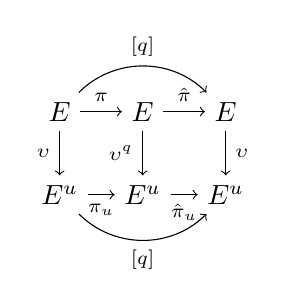
\begin{tikzpicture}[node distance=3em]
      \node(E){$E$};
      \node[right of=E](E2){$E$};
      \node[right of=E2](E3){$E$};
      \node[below of=E](Eu){$E^u$};
      \node[right of=Eu](Eu2){$E^u$};
      \node[right of=Eu2](Eu3){$E^u$};

      \draw[->,auto,font=\scriptsize]
      (E) edge node[swap]{$\upsilon$} (Eu)
          edge node{$\pi$} (E2)
          edge[bend left=45] node{$[q]$} (E3)
      (Eu) edge node[swap]{$\pi_u$} (Eu2)
           edge[bend right=45] node[swap]{$[q]$} (Eu3)
      (E2) edge node[swap]{$\upsilon^q$} (Eu2)
           edge node{$\hat\pi$} (E3)
      (Eu2) edge node[swap]{$\hat\pi_u$} (Eu3)
      (E3) edge node{$\upsilon$} (Eu3);
    \end{tikzpicture}
  \end{equation*}
  where we denote by $\upsilon^q$ the isomorphism
  $(x,y)\mapsto(u^{2q}x,u^{3q}y)$, and by $\hat\pi,\hat\pi_u$ the dual isogenies
  to $\pi,\pi_u$.

  Now we restrict the maps above to the $q$-torsion subgroups of $E$
  and $E^u$. Since the curves are ordinary, these subgroups are cyclic
  of order $q$, and the maps act as scalar multiplication on the
  points. In particular, we deduce from Eq.~\eqref{eq:frob-char-twist} that 
  \begin{equation*}
    \pi = [t \bmod q], \qquad \pi_u = [t_u \bmod q].
  \end{equation*}
  Hence, from the diagram we obtain
  \begin{equation*}
    [t] = \upsilon^{-q}\circ[t_u]\circ\upsilon \mod q.
  \end{equation*}

  Notice that $\upsilon^{-q}$ can be decomposed as
  $\upsilon^{-1}\circ\upsilon^{1-q}$, where $\upsilon^{1-q}$ is an
  automorphism of $E^u$ by hypothesis. $\upsilon^{1-q}$ also acts on
  the $q$-torsion points as a scalar in $\Z/q\Z$, that we shall denote
  by $U$. It is evident that the multiplicative order of $U$ in $\Z/q\Z$
  is the same as that of $u^{1-q}$ in $\F_p$. Then
  \begin{equation*}
    [t] = \upsilon^{-1}\circ[Ut_u]\circ\upsilon\mod q.
  \end{equation*}
  But $\upsilon$ is an isomorphism, thus it commutes with scalar
  multiplication, and we conclude that $t=Ut_u\bmod q$.

  If $u^{1-q}=\pm1$, we are done. When the order of $u^{1-q}$ is $3,4$
  or $6$, we still have to determine which of the cubic, fourth, sixth
  roots of unity in $\Z/q\Z$ corresponds to $U$.

  Using the diagram above, we decompose
  Eq.~\eqref{eq:frob-char-twist} as
  \begin{equation*}
    \hat\pi\circ\pi = [t]\pi - \pi^2,
  \end{equation*}
  and similarly for $E^u$. Hence, from the diagram again,
  \begin{equation}
    \label{eq:twisttrace:modp}
    [t] - \pi = \hat\pi = \upsilon^{-1}\circ\hat\pi_u\circ\upsilon^q 
    =  \upsilon^{-1}\circ([t_u] - \pi_u)\circ\upsilon^q.
  \end{equation}
  Let now $\omega$ be the invariant differential of $E$, we apply the
  pullback of Eq.~\eqref{eq:twisttrace:modp} to $\omega$. On the
  left-hand side we have
  \begin{equation}
    \label{eq:twisttrace:modp-lhs}
    ([t]-\pi)^\ast\omega = t\omega\in\Omega_E
  \end{equation}
  because $\pi$ is inserparable (see \cite[\S~5]{Sil}). On the
  right-hand side, if we let $\omega_u$ be the invariant differential
  of $E^u$, we have $(\upsilon^{-1})^\ast\omega=u\omega_u$, and
  $(\upsilon^q)^\ast\omega_u=\omega/u^q$, hence
  \begin{equation}
    \label{eq:twisttrace:modp-rhs}
    (\upsilon^{-1}\circ([t_u] - \pi_u)\circ\upsilon^q)^\ast\omega =
    u(([t_u] - \pi_u)\circ\upsilon^q)^\ast\omega_u =
    ut_u(\upsilon^q)^\ast\omega_u = u^{1-q}t_u\omega.
  \end{equation}
  Comparing Eqs.~\eqref{eq:twisttrace:modp-lhs}
  and~\eqref{eq:twisttrace:modp-rhs}, we conclude that $t = u^{1-q}t_u
  \bmod p$. Given that $\lvert t_u\rvert\le2\sqrt{q}$, we have uniquely determined $t_u$, and proven the theorem.
\end{proof}

\todo{Give a similar proposition for supersingular curves (see, e.g.,
  Menezes-Okamoto-Vanstone)}

%%%%%%%%%%%%%%%%%%%%%%%%%%%%%%%%%%
%%%%%%%%%%%%%%%%%%%%%%%%%%%%%%%%%%

\bibliographystyle{plain}
\bibliography{defeo}

\end{document}


% Local Variables:
% ispell-local-dictionary:"american"
% End:

%  LocalWords:  isomorphism cyclotomic coprime subfield Frobenius
%  LocalWords:  endomorphism eigenspace
